\documentclass[11pt,letterpaper]{article}
\usepackage[margin=1in,headheight=15pt]{geometry}
\usepackage[T1]{fontenc}
\usepackage{newpxtext}
\usepackage{amsmath,amsthm,mathtools}
\usepackage{newpxmath}
\usepackage{microtype}
\usepackage[table]{xcolor}
\usepackage{booktabs,tabularx,array,longtable}
\usepackage{enumitem}
\usepackage{tikz}
\usetikzlibrary{positioning,arrows.meta}
\usepackage[most]{tcolorbox}
\usepackage{listings}
\usepackage{fancyhdr}
\usepackage{titlesec}
\usepackage{hyperref}
\usepackage{bookmark}
\definecolor{forest}{HTML}{264B3D}
\definecolor{olive}{HTML}{737A43}
\definecolor{sage}{HTML}{EDF2EC}
\definecolor{ink}{HTML}{23312C}
\definecolor{muted}{HTML}{5C6860}
\hypersetup{colorlinks=true,linkcolor=forest,citecolor=forest,urlcolor=forest,
 pdftitle={Friendly Order Types of Finite Posets and Ordinal Products: Incomparability Components, Forest Certificates, and Exact Transfinite Formulas},
 pdfauthor={ChatGPT, research report prepared for Vladimir Reshetnikov},
 pdfsubject={Exact formulas, forest certificates, and a compositionality obstruction for the friendly order type},
 pdfkeywords={well-partial-order, friendly order type, incomparability graph, graphic matroid, ordinal product, natural product, lexicographic substitution, generating function}}
\titleformat{\section}{\Large\bfseries\color{forest}}{\thesection}{0.7em}{}
\titleformat{\subsection}{\large\bfseries\color{forest}}{\thesubsection}{0.7em}{}
\titleformat{\subsubsection}{\normalsize\bfseries\color{forest}}{\thesubsubsection}{0.7em}{}
\titlespacing*{\section}{0pt}{2.5ex plus 1ex minus .2ex}{1.1ex}
\titlespacing*{\subsection}{0pt}{1.8ex plus .8ex minus .2ex}{.7ex}
\pagestyle{fancy}
\fancyhf{}
\fancyhead[L]{\small\color{muted}\textsc{Friendly order types}}
\fancyhead[R]{\small\color{muted}Research report / 19 September 2026}
\fancyfoot[C]{\color{forest}\thepage}
\renewcommand{\headrulewidth}{0.3pt}
\renewcommand{\footrulewidth}{0pt}
\setlength{\parskip}{.35em}
\setlength{\parindent}{1.1em}
\setcounter{tocdepth}{1}
\setlist{itemsep=.25em,topsep=.4em}
\newtheorem{theorem}{Theorem}[section]
\newtheorem{lemma}[theorem]{Lemma}
\newtheorem{proposition}[theorem]{Proposition}
\newtheorem{corollary}[theorem]{Corollary}
\theoremstyle{definition}
\newtheorem{definition}[theorem]{Definition}
\newtheorem{example}[theorem]{Example}
\newtheorem{question}[theorem]{Question}
\newtheorem{problem}[theorem]{Problem}
\theoremstyle{remark}
\newtheorem{remark}[theorem]{Remark}
\newcommand{\fot}{f}
\newcommand{\mot}{o}
\newcommand{\str}{\operatorname{str}}
\newcommand{\pred}{\operatorname{pred}}
\newcommand{\Bad}{\operatorname{Bad}}
\newcommand{\Fr}{\operatorname{Fr}}
\newcommand{\Inc}{\operatorname{Inc}}
\newcommand{\Min}{\operatorname{Min}}
\newcommand{\rk}{\operatorname{rk}}
\newcommand{\res}[2]{#1_{\not\ge #2}}
\newcommand{\N}{\mathbb{N}}
\newcommand{\epsmin}{\varepsilon_{\min}}
\newcommand{\epsmax}{\varepsilon_{\max}}
\newcommand{\epsbot}{\varepsilon_{\bot}}
\newcommand{\epstop}{\varepsilon_{\top}}
\newcommand{\wpo}{\textnormal{wpo}}
\newcommand{\one}{\mathbf{1}}
\newcommand{\chain}[1]{\mathbf{#1}}
\newcommand{\anti}[1]{\Gamma_{#1}}
\newcommand{\Bool}{\mathcal{B}}
\newcommand{\gfA}{\mathsf{A}}
\newcommand{\gfB}{\mathsf{B}}
\newtcolorbox{resultbox}[1][]{colback=sage,colframe=forest,boxrule=.5pt,
 arc=1.5mm,left=3mm,right=3mm,top=2mm,bottom=2mm,breakable,#1}
\lstset{basicstyle=\small\ttfamily,columns=fullflexible,keepspaces=true,
 breaklines=true,frame=single,rulecolor=\color{olive},backgroundcolor=\color{sage},
 showstringspaces=false,aboveskip=.8em,belowskip=.8em}
\newcolumntype{Y}{>{\raggedright\arraybackslash}X}
\begin{document}
\begin{titlepage}
\color{ink}
\vspace*{-.35in}
{\small\bfseries\color{olive}\MakeUppercase{Order theory \enspace / \enspace Ordinal combinatorics}}
\par\vspace{.15in}
{\fontsize{27}{31}\selectfont\bfseries\color{forest}Friendly Order Types\par}
\vspace{.08in}
{\fontsize{25}{29}\selectfont\bfseries\color{forest}of Finite Posets and\par Ordinal Products\par}
\vspace{.12in}
{\fontsize{16}{20}\selectfont\bfseries\color{olive}Incomparability Components, Forest Certificates,\par
and Exact Transfinite Formulas\par}
\vspace{.16in}
{\large Exact formulas, composition laws, a compositionality obstruction,\par
forest certificates, and a finite-tail method\par}
\vspace{.12in}
\noindent\textcolor{olive}{\rule{\textwidth}{1pt}}
\vspace{.10in}
\noindent\textbf{Research report}\hfill 19 September 2026\\[.35em]
Prepared for Vladimir Reshetnikov \hfill Prepared by ChatGPT
\vspace{.09in}
\begin{resultbox}[title={\bfseries Main conclusions}]
\small
For a finite poset $P$, let $c(P)$ count the connected components of its
incomparability graph $\Inc(P)$, including isolated vertices. Then
\[
 \fot(P)=|P|-c(P),
 \qquad\text{equivalently}\qquad
 w\bigl(M^r(P)\bigr)=\omega^{|P|-c(P)}.
\]
So $\fot(P)$ is the rank of the graphic matroid of $\Inc(P)$. The optimal
sequences are classified and carry spanning-forest certificates.

For a non-chain finite Cartesian product of ordinals, and more generally for
a product of infinite ordinals with an arbitrary finite poset, the friendly
order type equals the natural product, except that one rightmost successor is
removed when every ordinal factor is a successor and the finite factor has a
greatest element.

Two four-element posets with identical $(o,h,w,f)$ give different friendly
order types after multiplication by the same two-element chain, so those four
invariants do not support a general product formula.
\end{resultbox}
\vspace{.10in}
\footnotesize
\noindent\textbf{Abstract.}
The compositional calculation of friendly order type is an explicitly
identified research direction in work of Isa Vialard. We prove that for a
finite poset the invariant is exactly the rank of the graphic matroid of the
incomparability graph. The key lemma produces a maximal non-cut vertex while
protecting any prescribed minimal root; it yields optimal sequences,
spanning-forest certificates, and a classification of all maximum friendly
subsets. From the formula we derive composition laws for ordinal sums,
disjoint unions, lexicographic substitutions and Cartesian products (proved
twice, by two independent routes), and an exact bivariate generating function
for the distribution on naturally labelled posets. We then study finite
successor tails of ordinal products: a projection argument shows that a
nontrivial Cartesian product has a single non-endpoint incomparability
component, and isolating the finite upper corner of an infinite ordinal
product yields exact transfinite formulas rather than finite approximations.
Well-ordered sums of two-element antichains realize every ordinal, even
though all countably infinite instances have isomorphic incomparability
graphs. The software compares the defining recursion with the formula on
$101{,}660$ naturally labelled posets through size seven.
\vfill
\end{titlepage}

\tableofcontents
\vspace{1em}
\begin{resultbox}[title={\bfseries Reading guide}]
Sections~\ref{sec:finite}--\ref{sec:counterexample} are finite and elementary;
the component formula can be checked by reading only
Sections~\ref{sec:preliminaries}--\ref{sec:finite}, with no transfinite
notation. Section~\ref{sec:subsets} classifies the optimal witnesses and
gives the matroid reading. Sections~\ref{sec:tails}--\ref{sec:mixed} contain
the transfinite argument. The complete classification of ordinal boxes is in
Theorem~\ref{thm:boxes}; the transfinite sum law and the realization of every
ordinal are in Section~\ref{sec:sums}; Section~\ref{sec:enumeration} counts
naturally labelled posets by their friendly rank.
Section~\ref{sec:computation} and the appendices explain exactly what the
software verifies and what it does not verify.
\end{resultbox}

\vspace{.6em}
\begin{resultbox}[title={\bfseries Status and scope}]
\small
Conventional proofs are supplied for the results developed here; the
transfinite argument uses explicitly cited published theorems, and
Appendix~\ref{app:ledger} separates imported statements from those proved
below. The arguments are presented as proofs, but this is a research draft:
it has not been independently refereed, formally verified, or checked by a
proof assistant. A literature search located neither the component formula
nor the exact transfinite formulas, but that is not a certification of
priority, the elementary ingredients may be known in other terminology, and
no publication-priority claim is made. The invariant itself, the
multiset-width transfer, the both-limit product case and the binary
ordinal-sum law are Vialard's and are not claimed as new. This report
resolves the finite specialization, the ordinal-product family and a class of
well-ordered sums; it does not resolve the unrestricted compositional program
for arbitrary well-partial-orders, and it proves no formula for infinite
connected pieces.
\end{resultbox}

\vspace{.6em}
\begin{resultbox}[title={\bfseries Provenance}]
\small
This report is a merge of two independently produced research reports on the
same invariant, originally delivered as the directories
\texttt{cartesian-products-of-ordinals} and
\texttt{incomparability-components-and-forests}. The first developed the
transfinite side: the ordinal-cut projection lemma, the finite-tail and
upper-tail lemmas, the mixed ordinal--finite product theorem, the complete
classification of ordinal boxes, and the $(o,h,w,f)$ counterexample. The
second developed the finite side: the protected-root strengthening of the
deletion lemma, the classification of maximum friendly subsets, the
spanning-forest certificates and the graphic-matroid reading, the
substitution and disjoint-union laws, the enumerative generating function,
and the infinite graph-only obstruction.

Both reports independently proved the shared core theorem
$\fot(P)=|P|-c(P)$, and they proved it by the same argument: the same
ordered-component lemma, the same maximal non-cut vertex lemma with the same
two-case proof, the same component-capacity upper bound, and the same
top-down assembly. That argument is therefore given exactly once below, in
Section~\ref{sec:finite}; the second report's protected-root strengthening
of Lemma~\ref{lem:noncut} is retained, since the classification of maximum
friendly subsets needs it. Where the two reports genuinely differed, both are
kept: the finite Cartesian-product formula is proved twice, once by the
ordinal-cut projection route of Section~\ref{sec:products} and once by the
chain-grid spanning-subgraph route of Section~\ref{sec:grid-proof}.
\end{resultbox}
\clearpage

\section{The selected problem and its scope}\label{sec:scope}

\subsection{A documented open direction}
Vialard introduced the friendly order type $o_\perp(P)$ in the study of
ordinal widths of finite multiset orderings. The conclusion of the MFCS
2023 paper asks about further compositional calculations of this invariant
\cite[Conclusion, p.~87:11]{Vialard2023}. The conclusion of the subsequent
thesis again presents its compositional computation as a research direction
\cite[Conclusion, p.~109]{VialardThesis}. We write $f(P)$ instead of
$o_\perp(P)$ throughout this report.

The broad question needs a precise interpretation. A construction may be
computable from a rich structural description of its inputs without being
a function of a short list of their ordinal invariants. These are different
notions of compositionality. We investigate both, through the following
restricted questions.

\begin{question}\label{q:finite}
Can the friendly order type of an arbitrary finite poset be recovered
from a simple structural statistic, without constructing its entire
friendly bad-sequence tree?
\end{question}

\begin{question}\label{q:scalar}
Is $f(A\times B)$ determined by the two tuples
\[
 (o(A),h(A),w(A),f(A))\quad\text{and}\quad(o(B),h(B),w(B),f(B))?
\]
\end{question}

\begin{question}\label{q:ordinal}
Can one compute $f(P)$ exactly when $P$ is a finite product of ordinals,
or more generally a product of infinite ordinals with a finite poset?
\end{question}

Question~\ref{q:finite} is the finite specialization of the published
direction, and it is worth stating separately in the sharper form we actually
answer.

\begin{problem}[Finite specialization]\label{prob:finite}
Given an arbitrary finite poset $P$, identify a nonrecursive structural
expression for its friendly order type. Use that expression to obtain
composition laws and explicit optimal witnesses.
\end{problem}

These precise questions are formulations adopted in this report; we do
not attribute them verbatim to Vialard, and we do not claim that the
literature separately labels the finite statement as a named conjecture.
We answer the first and third positively and the second negatively. This
resolves specified subproblems of the published program, not the
unrestricted program for arbitrary well-partial-orders and arbitrary
constructions.

\subsection{What was already known}
The limit-ordinal case must not be mistaken for a new result. Vialard's
thesis already proves
\[
 f(A\times B)=o(A\times B)
 \quad\text{if both $o(A)$ and $o(B)$ are limit ordinals}
\]
\cite[Theorem~5.4.8(3)]{VialardThesis}.
The binary ordinal-sum rule is also known
\cite[Proposition~4.1(1)]{Vialard2023}. The invariant itself, and its
connection to multiset width, are due to Vialard
\cite[Definition~3.3, Theorem~3.4]{Vialard2023}. None of this may be
represented as a discovery of this report. We use these facts for context,
not as claims of novelty. Our transfinite proof rests on the published
limit-saturation theorem stated in Section~\ref{sec:preliminaries}; the
additional work is to control stripping and the finite successor corner
exactly. The finite disjoint-union identity of
Corollary~\ref{cor:finite-sums} is likewise not claimed as a new special
case; what is contributed there is its common structural explanation.

\subsection{What this report establishes}
Theorem~\ref{thm:finite} gives the finite formula $f(P)=|P|-c(P)$, and
Corollary~\ref{cor:graphic} reads it as the rank of the graphic matroid of
the incomparability graph. Theorem~\ref{thm:subsets} classifies every
maximum friendly subset, and Proposition~\ref{prop:forest} attaches a
spanning-forest certificate to the constructed witnesses.
Theorem~\ref{thm:product-components} identifies the incomparability
components of every Cartesian product with two non-singleton factors, giving
the product formula of Corollary~\ref{cor:finite-product}; that formula is
proved a second time, by an independent graph-theoretic route, in
Section~\ref{sec:grid-proof}. Theorem~\ref{thm:substitution} gives an exact
formula for arbitrary nonempty finite lexicographic substitutions.
Theorem~\ref{thm:no-scalar} gives an explicit counterexample to
Question~\ref{q:scalar}. Theorem~\ref{thm:mixed} settles the mixed
ordinal--finite product problem, including the distinction between a
finite factor with and without a greatest element.
Theorem~\ref{thm:ordinal-sum} gives the transfinite sum law, from which
Corollary~\ref{cor:all-ordinals} realizes every ordinal as a friendly order
type at ordinary antichain width two, while
Proposition~\ref{prop:graph-obstruction} shows that on infinite wpos the
graph alone no longer determines the invariant.
Theorem~\ref{thm:gf} computes the exact bivariate generating function for
the distribution on naturally labelled posets.

A useful feature is that the strongest theorem is not restricted to
countable ordinals. The proofs take place in ZFC and apply to arbitrary
set-sized ordinals. The executable ordinal notation system is deliberately
more restricted: it handles ordinals below $\varepsilon_0$, which admit
finite hereditary Cantor normal forms.

\subsection{Literature and novelty status}
The source check for this report was made on 19 September 2026. It included
the official MFCS proceedings version, the author-hosted thesis, the earlier
arXiv version, the author's publication list, and exact-phrase searches for
the invariant under its published and earlier terminology and for an
incomparability-component formula
\cite{Vialard2023,VialardThesis,VialardPreprint,VialardWebsite}. The
prepublication arXiv version uses ``maximal safe order type''; definitions
and citations here follow the published friendly-order-type treatment.
General infinite formulas not used in our proofs are deliberately not
imported from earlier source versions.

The exact finite formula, the particular obstruction, and the complete
successor-tail calculation below were not located in the sources checked.
That is a limited literature-search conclusion, not a proof of priority, and
not a guarantee that no later solution exists. The elementary ingredients
may be known in other terminology. The appropriate status is:
\emph{results proved in this draft, with independent expert review and a
fuller novelty check still desirable}. The mathematical assertions below have
explicit proofs independent of any assertion of novelty; if the component
formula turns out to be implicit in an earlier source, the proofs and
artifacts remain useful but the novelty statement would need revision.
That question is separate from the question whether the displayed theorems
follow from the arguments given. The argument is not presented as a
resolution of an unrelated famous conjecture, nor is computational agreement
presented as a transfinite proof.

\section{Definitions and proof dependencies}\label{sec:preliminaries}

\subsection{Well-partial-orders and residuals}
A finite or infinite sequence $x_0,x_1,\ldots$ in a poset $P$ is
\emph{bad} if there is no pair $i<j$ with $x_i\le x_j$. A
\emph{well-partial-order}, abbreviated wpo, has no infinite bad sequence.
For $x\in P$, write
\[
 \uparrow x=\{y\in P:x\le y\},\qquad
 \res P x=P\setminus\uparrow x.
\]
For a finite sequence $s$, the residual is
\[
 \res P s=P\setminus\bigcup_{x\text{ occurring in }s}\uparrow x.
\]
Every next term of a bad sequence belongs to the current residual.
All orders on subsets in this report are induced orders.

A well-founded tree has rank given recursively by
\begin{equation}\label{eq:tree-rank}
 \rk(s)
 =\sup\{\rk(s^{\frown}x)+1:s^{\frown}x\text{ is in the tree}\},
 \qquad\sup\varnothing=0,
\end{equation}
where the supremum of the empty set is zero. The tree rank is the rank of
the empty sequence. In a finite tree it is the maximum number of edges on a
root-to-leaf path. In general it need not be the supremum of the finite
lengths of its branches; this distinction will be essential. These are the
standard rank conventions for ordinal invariants of well-quasi-orders
\cite{DSS}.

\subsection{The friendly restriction}
Two points are \emph{incomparable}, written $x\perp y$, when neither is
below the other. The \emph{incomparability graph} $\Inc(P)$ has vertex set
$P$ and an undirected edge between distinct incomparable elements. A bad
sequence is \emph{friendly} (called open-ended in the original definition)
if, when each term $x$ is selected, the current residual contains a point
$y\perp x$. The point $y$ is a friend witnessing that move. This is the
definition from \cite[Definition~5.3.2]{VialardThesis}, published as
\cite[Definition~3.3]{Vialard2023}, where the invariant is written
$o_\perp(P)$.

The empty sequence is friendly. The friend is required in the residual
\emph{before} the choice is made; being incomparable with $x$, it survives
that individual choice, but it need not survive later choices and need not
ever be selected. These distinctions matter: requiring a permanent friend,
or requiring only a friend in the original poset, would define different
processes. Let $\Fr(P)$ be the tree of friendly bad sequences, and
let $f(P)$ be its rank. Equivalently,
\begin{equation}\label{eq:f-residual}
 f(P)=\sup_{\substack{x\in P\\ \exists y\in P\ (x\perp y)}}
       \bigl(f(\res P x)+1\bigr).
\end{equation}
For a finite poset this rank is the maximum number of legal moves. For an
infinite wpo it is an ordinal rank, not an infinite play: all individual
plays remain finite.

\begin{lemma}[Basic properties]\label{lem:basic}
For wpos $S\subseteq P$, with induced order,
\[
 f(S)\le f(P),\qquad f(P)\le o(P).
\]
Also $f(P)=0$ exactly when $P$ is a chain, including the empty chain.
If a legal sequence of $k$ moves leaves residual $R$, then
\begin{equation}\label{eq:moves}
 f(P)\ge f(R)+k.
\end{equation}
The addition in this formula is ordinary ordinal addition on the right.
Finally, every subsequence of a friendly sequence is friendly.
\end{lemma}
\begin{proof}
A friendly sequence in $S$, with its friends in $S$, remains friendly in
$P$: an earlier selected point removes precisely the same points of $S$
in either ambient poset. Thus $\Fr(S)$ is a subtree of $\Fr(P)$.
The friendly tree is a subtree of the full bad-sequence tree, which gives
the second inequality. Equation~\eqref{eq:f-residual} has an eligible first
move exactly when an incomparable pair exists. Next apply
\eqref{eq:f-residual} successively along the specified legal sequence.
Each step adds a successor on the right, so after $k$ steps the lower
bound is $f(R)+k$.

For the last assertion, deleting earlier choices from a friendly sequence
only enlarges each subsequent residual, and it removes no comparison. The
friends witnessing the original sequence therefore witness the subsequence
as well.
\end{proof}

For a finite nonempty poset with $n$ elements one has the elementary bound
\begin{equation}\label{eq:rough-bound}
 0\le f(P)\le n-1.
\end{equation}
Indeed, all selected points are distinct, and the last selected point needs
a different point still present as a friend. The task of
Section~\ref{sec:finite} is to determine exactly how much stronger this bound
becomes when the incomparability graph is disconnected.

\subsection{The stripped poset}
Define
\[
 \str(P)=\{x\in P:\exists y\in P\ (x\perp y)\}.
\]
It removes every point comparable with all points of $P$. Every selected
point of a friendly sequence belongs to $\str(P)$, so
\begin{equation}\label{eq:strip-upper}
 f(P)\le o(\str(P)).
\end{equation}
Notice that stripping can remove more than endpoints in a general poset.
The fact that products behave much better is one of the main structural
lemmas of this report.

\subsection{Imported theorems}
We explicitly isolate the external results used in the transfinite part.
The maximal order type $o(P)$ is the rank of the bad-sequence tree. The
maximal-linearization theorem of de Jongh and Parikh identifies it with an
\emph{attained} maximum among order types of well-order linear extensions.
For wpos $A,B$,
\begin{equation}\label{eq:mot-product}
 o(A\times B)=o(A)\otimes o(B),
\end{equation}
where $\otimes$ is the natural product \cite{DeJonghParikh}.
The use of an attained maximum, rather than just a supremum, matters in
Lemma~\ref{lem:upper-tail}.

\begin{theorem}[Published limit saturation]\label{thm:imported-limit}
If $P$ is a wpo, $o(P)$ is a nonzero limit ordinal, and
$o(\str(P))=o(P)$, then
\[
 f(P)=o(P).
\]
\end{theorem}
This is Vialard's Corollary~4.7 \cite{Vialard2023}. Its proof is not
reproduced here. Accordingly, our transfinite proofs are complete
\emph{relative to this explicitly stated published theorem}, not a new
self-contained derivation of the entire underlying theory.

A second imported result supplies a useful application. A finite multiset on
$P$ is a finitely supported function $P\to\N$. Let $M^r(P)$ be the set of
finite multisets with the multiset ordering: for multisets $\mu,\nu$, cancel
their common part; then $\mu<_r\nu$ when the remainder of $\nu$ is nonempty
and every occurrence remaining in $\mu$ is strictly below some occurrence
remaining in $\nu$. A single witness in $\nu$ may be reused for several
occurrences, so the domination need not be injective. Adding equality gives
$\le_r$. This is \emph{not} the distinct, injective multiset embedding order
\cite[Section~1]{Vialard2023}. Vialard proves
\begin{equation}\label{eq:multiset}
 w(M^r(P))=\omega^{f(P)}
\end{equation}
for every wpo $P$
\cite[Theorem~3.4]{Vialard2023}, restated as
\cite[Definition~5.3.2, Theorem~5.3.3]{VialardThesis}. Its technical proof
is neither reproduced nor claimed as new here. We use \eqref{eq:multiset}
only for consequences, not for any main proof; all computations of its
exponent below come from the self-contained finite argument.

The ordinal height and width are the ranks, under the convention
\eqref{eq:tree-rank}, of the trees of strictly decreasing sequences and of
sequences of pairwise incomparable elements, respectively. For finite posets
they are the ordinary largest chain and antichain cardinalities. For infinite
wpos, ordinal width is not simply the supremum of finite antichain sizes,
and it may be a transfinite ordinal.

\section{Every finite poset: a component formula}\label{sec:finite}

\subsection{Incomparability components are ordered blocks}
Write $c(P)$ for the number of connected components of $\Inc(P)$ when $P$ is
finite, counting isolated vertices. Put $c(\varnothing)=0$: the empty graph
has zero components. When the graph rather than the poset is in focus we also
write $c(\Inc(P))$ for the same number.

Recall that the \emph{ordinal sum} $A+B$ retains the internal orders of $A$
and $B$ and places every element of $A$ below every element of $B$, whereas
the \emph{disjoint union} $A\sqcup B$ adds no cross comparisons at all.
These two operations behave completely differently here, and the distinction
is used throughout.

\begin{lemma}[Ordered components]\label{lem:ordered-components}
Distinct connected components of $\Inc(P)$ are uniformly comparable.
They therefore form linearly ordered ordinal-sum blocks: for two distinct
components $C,D$, either every point of $C$ is below every point of $D$,
or every point of $D$ is below every point of $C$.
\end{lemma}
\begin{proof}
Points in distinct components must be comparable, since otherwise they
would be adjacent. Suppose $x\perp x'$ lie in one component and $z$ lies
in another. Opposite orientations, such as $x<z<x'$, contradict
$x\perp x'$. Thus the orientation of comparison with $z$ is constant
along every incomparability edge and hence along every path. Applying the
same argument to paths in the second component gives uniform comparison
between the two components. Transitivity and antisymmetry of $P$ make the
resulting comparison a linear order on the set of components.
\end{proof}

For a wpo the component order is itself a well-order: an infinite
descending sequence of components, with one representative from each,
would give an infinite strictly descending sequence in $P$. For the finite
theorem we need only the elementary finite version of this observation.

In particular, every finite poset has a canonical decomposition
\begin{equation}\label{eq:component-sum}
 P=C_1+C_2+\cdots+C_c
\end{equation}
as an ordinal sum of its incomparability components in increasing order.
This is a decomposition into \emph{induced} posets. It does not assert that
the components are chains or antichains; they are arbitrary posets with
connected incomparability graph. Nor is it a disjoint union: the blocks in
\eqref{eq:component-sum} are completely comparable to one another.

\subsection{The capacity of a single component}

\begin{lemma}[Component capacity]\label{lem:capacity}
In any friendly sequence in a finite poset, at most $|C|-1$ points can be
selected from each incomparability component $C$.
\end{lemma}
\begin{proof}
A friend of a point of $C$ must also lie in $C$, since an incomparability
edge cannot join distinct components. Suppose a sequence selected every point
of $C$, and consider its last choice from $C$. All other points of $C$ would
already have been selected, hence already removed, so no friend could remain
in the residual. This contradicts the friend condition. Points removed
incidentally, without being selected, only shrink the residual further and
cannot repair the obstruction.
\end{proof}

\begin{corollary}[Component upper bound]\label{cor:upper}
For every finite poset,
\[
 f(P)\le|P|-c(P).
\]
\end{corollary}
\begin{proof}
Apply Lemma~\ref{lem:capacity} to each of the $c(P)$ components and add.
Equivalently, each component contains a point that is never selected.
The argument distinguishes points that are \emph{selected} from points
removed incidentally; it does not confuse these two events.
\end{proof}

The real issue is the lower bound: can these local capacities all be reached
simultaneously? A generic graph deletion order does not suffice, because
deleting an upward closure can remove several vertices at once. To avoid
losing points that have not been selected, the next selected vertex should be
maximal in the remaining poset. The next lemma supplies exactly this.

\subsection{A maximal point can be deleted without disconnecting}

A vertex of a graph is \emph{non-cut} if deleting it leaves a connected
graph. We apply this only to connected graphs with at least two vertices;
the one-vertex graph left after a deletion counts as connected. The lemma
below is stated in the strengthened form we shall need later: the vertex it
produces can be kept away from any prescribed minimal element. That
strengthening costs only two extra clauses in the same proof, and
Theorem~\ref{thm:subsets} depends on it.

\begin{lemma}[Maximal non-cut vertex with a protected root]\label{lem:noncut}
Let $P$ be finite with $|P|>1$ and $\Inc(P)$ connected, and let $r$ be any
minimal element of $P$. Then $P$ has a maximal element $v\ne r$ such that
$\Inc(P\setminus\{v\})$ is connected. In particular, taking $r$ to be an
arbitrary minimal element, $P$ has a maximal non-cut vertex.
\end{lemma}
\begin{proof}
Choose a maximal element $u\ne r$. Such a $u$ exists: if $r$ were the only
maximal element, finiteness would put every element below $r$, contradicting
the minimality of $r$ together with $|P|\ge2$. If deleting $u$ leaves a
connected graph, take $v=u$ and stop.

Otherwise, by Lemma~\ref{lem:ordered-components},
the components of $P\setminus\{u\}$ can be written
\[
 C_1<C_2<\cdots<C_k,\qquad k\ge2.
\]
Connectivity of $\Inc(P)$ forces $u$ to have a neighbor in every $C_i$:
otherwise $C_i$ would have no edge to $u$ and none to any other $C_j$.
Choose $a\in C_1$ with $a\perp u$.

For $z\in C_j$ with $j>1$, we have $a<z$. The relation $z<u$ would imply
$a<u$, while $u<z$ contradicts maximality of $u$. Thus
\begin{equation}\label{eq:u-universal}
 u\perp z\quad\text{for every }z\in C_2\cup\cdots\cup C_k.
\end{equation}
Choose a maximal element $v$ of $C_k$. It is maximal in $P$: nothing in an
earlier component can be above it, nothing in $C_k$ is strictly above it,
and $u$ is incomparable with it. Moreover $v\ne r$: every element of $C_1$
lies below $v$, while $r$ is minimal in $P$.

After deleting $v$, all the earlier components remain connected internally
and attached to $u$. Every surviving vertex of $C_k$ is directly adjacent
to $u$ by \eqref{eq:u-universal}, whether or not deleting $v$ disconnects
the graph inside $C_k$. If $C_k=\{v\}$, this last requirement is
vacuous. The remaining graph is connected in either case.
\end{proof}

The order-theoretic word ``maximal'' is important, and it is the point at
which transitivity of the order supplies more than graph connectivity alone.
A connected graph always has non-cut vertices, but an arbitrary non-cut
vertex need not delete only itself under the friendly residual operation:
deleting an upward closure could remove several vertices at once and destroy
the intended sequence length. A maximal point does delete only itself,
because its principal upper set within the current component is a singleton.

\begin{proposition}[Connected case]\label{prop:connected}
For a finite nonempty poset with connected incomparability graph,
\[
 f(P)=|P|-1.
\]
More strongly, for every minimal $r\in P$ there is a friendly sequence
selecting precisely $P\setminus\{r\}$. At each step it selects a maximal
vertex of the current induced poset and leaves that poset's incomparability
graph connected.
\end{proposition}
\begin{proof}
A singleton gives the empty sequence. For at least two elements, apply
Lemma~\ref{lem:noncut} with protected root $r$. The chosen $v$ has a friend,
since the graph is connected with more than one vertex. Since $v$ is maximal,
its upward closure in the current poset is $\{v\}$, so the residual is
exactly $P\setminus\{v\}$, again with connected incomparability graph, and
$r$ is still minimal in it. Induction repeats the construction until only
$r$ remains, making $|P|-1$ moves.

Optimality is \eqref{eq:rough-bound}, or equally
Corollary~\ref{cor:upper} with $c(P)=1$: no friendly sequence can select
every point of a nonempty finite poset, since the final selected point would
require an available incomparable point not already selected.
\end{proof}

\subsection{The exact formula}

\begin{theorem}[Finite friendly order type]\label{thm:finite}
For every finite poset $P$,
\begin{equation}\label{eq:finite-formula}
 \boxed{f(P)=|P|-c(P).}
\end{equation}
\end{theorem}
\begin{proof}
The empty case is immediate. Write the canonical decomposition
\eqref{eq:component-sum} as $P=C_1+\cdots+C_c$.

The upper bound is Corollary~\ref{cor:upper}.

For the lower bound, choose a minimal root $r_i$ in each induced component
$C_i$, and use Proposition~\ref{prop:connected} to obtain, inside $C_i$, a
local friendly sequence of length $|C_i|-1$ leaving only $r_i$ in that
component. Run these local sequences in the order $C_c,C_{c-1},\ldots,C_1$.
A move in a higher component never removes a point of a lower component, so
each component is still intact when its local sequence starts. A move in a
lower component may remove surviving roots of higher components, but those
roots are no longer needed: every local friend lies in the component
currently being processed. The friends and maximal deletions inside the
current component therefore remain valid, and the concatenated sequence is
legal with length
\[
 \sum_{i=1}^c(|C_i|-1)=|P|-c,
\]
completing the proof.
\end{proof}

\subsection{Sharp bounds in terms of the stripped cardinality}

\begin{corollary}\label{cor:finite-strip}
Let $s=|\str(P)|$ and let $k$ be the number of non-singleton
incomparability components of a finite poset $P$. Then
\begin{equation}\label{eq:strip-equality}
 f(P)=f(\str(P))=s-k.
\end{equation}
If $s=0$, then $f(P)=0$. The value $s=1$ is impossible. For every $s\ge2$,
\begin{equation}\label{eq:sharp-finite-bounds}
 \left\lceil\frac{s}{2}\right\rceil\le f(P)\le s-1,
\end{equation}
and every integer in this interval occurs.
\end{corollary}
\begin{proof}
Stripping removes exactly the isolated vertices of the incomparability
graph. Deleting one isolated vertex lowers the vertex count and the
component count by one, leaving their difference unchanged, so
Theorem~\ref{thm:finite} gives the equality $f(P)=f(\str(P))$ and the value
$s-k$. Note that this is an exact equality, sharper than the general upper
bound \eqref{eq:strip-upper}.

Each remaining component has at least two vertices. Thus
$1\le k\le\lfloor s/2\rfloor$ when $s>0$, and the formula gives the bounds.
For any allowed $k$, partition $s$ into $k$ integers at least two and take
an ordinal sum of antichains of those sizes. Its stripped cardinality is
$s$ and its friendly order type is $s-k$. This realizes every value.
\end{proof}

If instead one fixes only the cardinality and allows isolated vertices,
every value occurs: for an $n$-element poset, each integer $k$ with
$0\le k\le n-1$ is realized by $\chain{n-k-1}+\anti{k+1}$, with the
empty-chain convention when $k=n-1$. Here and below, $\chain m$ denotes an
$m$-element chain and $\anti m$ an $m$-element antichain.

\begin{proposition}[Exact monotonicity under augmentation]\label{prop:augment}
Let $P$ and $Q$ be finite posets on the same support, and suppose every
comparison of $P$ is also a comparison of $Q$. Then
\[
 f(P)-f(Q)=c(Q)-c(P)\ge0.
\]
\end{proposition}
\begin{proof}
Adding comparisons removes incomparability edges, and removing edges can
only split components, never join them; hence $c(Q)\ge c(P)$. Subtracting
the two instances of Theorem~\ref{thm:finite} gives the equality.
\end{proof}

The statement applies to the completed transitive order. Adding one proposed
comparison can force many others by transitivity, so a single new
comparison need not lower the invariant by exactly one.

For example, $f(\anti n)=n-1$ for a nonempty $n$-element antichain, while
$f(\chain n)=0$ for a chain. An ordinal sum of five two-element antichains
has ten stripped points but friendly order type five, whereas a ten-point
antichain has friendly order type nine. The arrangement into ordinal-sum
blocks, not simply the number of incomparable points, is decisive.

Combining Theorem~\ref{thm:finite} with the imported multiset identity gives
\begin{equation}\label{eq:finite-multiset}
 w(M^r(P))=\omega^{|P|-c(P)}
 \qquad(P\text{ finite}).
\end{equation}
The finite graph statistic therefore determines an infinite ordinal width.

The degenerate cases of \eqref{eq:finite-multiset} are worth keeping
explicitly. For $P=\varnothing$ there is exactly one multiset, the empty
one, so the width is $1=\omega^0$, not $0$; the formula gives the right
answer only because $f(\varnothing)=0$ and $\omega^0=1$. For a nonempty
finite chain the exponent is likewise zero, consistently with its multiset
ordering being a chain.

\section{Maximum friendly subsets and forest certificates}\label{sec:subsets}

Theorem~\ref{thm:finite} computes a rank. The construction behind it does
more: it identifies exactly which subsets of $P$ can be the set of selected
points of an optimal friendly sequence, and it equips each such sequence
with a certificate that can be checked without rerunning the search.

For a subset $S\subseteq P$ of a finite poset, say that $S$ is
\emph{friendly in $P$} if it admits a linear extension whose reverse listing
is a friendly bad sequence in $P$. By the last clause of
Lemma~\ref{lem:basic}, all subsequences of that listing are then friendly as
well. Conversely, a friendly sequence listing exactly the elements of $S$
has a reverse listing that is a linear extension of $S$: a selected point is
never above a point selected after it. This finite formulation agrees with
the friendly-subset condition used in Vialard's alternative
characterization \cite[Definition~4.4]{Vialard2023}.

\begin{theorem}[Classification of maximum friendly subsets]\label{thm:subsets}
Let $C_1<\cdots<C_c$ be the incomparability components of a finite poset
$P$. The friendly subsets of maximum possible size are exactly the sets
\begin{equation}\label{eq:subset-class}
 P\setminus\{r_1,\ldots,r_c\},\qquad r_i\in\Min(C_i),
\end{equation}
where $\Min(C_i)$ is the set of minimal elements of the induced poset
$C_i$. Their common size is $|P|-c$, and their number is
\begin{equation}\label{eq:subset-count}
 \prod_{i=1}^c|\Min(C_i)|,
\end{equation}
with the empty product equal to $1$.
\end{theorem}
\begin{proof}
The construction in Theorem~\ref{thm:finite} realizes every choice of roots
in \eqref{eq:subset-class}, because Proposition~\ref{prop:connected} accepts
an arbitrary prescribed minimal root of each component. This proves
sufficiency and the asserted size.

For necessity, a maximum friendly subset must omit at least one member of
each component by Lemma~\ref{lem:capacity}. Since its size is $|P|-c$, it
omits exactly one, say $r_i$, from each $C_i$. Fix a sequence listing the
subset and consider a component $C_i$. If $r_i$ were not minimal in $C_i$,
some selected $a\in C_i$ would satisfy $a<r_i$, so the root $r_i$ would be
removed at the choice of $a$. If that were not the last choice from $C_i$,
no unselected member of $C_i$ could remain as a friend for the last choice.
If it were the last choice, the only possibly remaining other member of
$C_i$ would be $r_i$ itself, which is comparable to $a$. Both possibilities
violate the friend condition, so each $r_i$ is minimal in its component.
Different root choices give different complements, so multiplying the
numbers of choices yields \eqref{eq:subset-count}.
\end{proof}

The theorem is stronger than a rank computation: it identifies every largest
witness subset. It does not enumerate all permissible orderings of a given
witness subset. Note also that the roots are minimal \emph{inside their own
component}, not necessarily minimal in $P$.

\begin{proposition}[Spanning-forest certificate]\label{prop:forest}
The construction in Theorem~\ref{thm:finite} can attach to every choice $x$
a friend $y$ such that the witness edges $\{x,y\}$ form a spanning tree in
each original incomparability component. The unselected roots $r_i$ are the
roots of those trees.
\end{proposition}
\begin{proof}
Within a component, choose as friend any neighbor remaining after deleting
the selected maximal vertex, and orient the witness edge from that vertex to
its friend. The endpoint is either selected later in that local sequence or
is the protected root. Following oriented edges therefore strictly increases
deletion time until the root is reached, so cycles are impossible. Every
non-root has exactly one outgoing edge and eventually reaches the root, so
the edges form a connected acyclic spanning subgraph of the component. The
construction never uses a friend from a different component, so on the whole
poset the witness edges form a spanning forest with one tree per component.
\end{proof}

\begin{corollary}[Graphic matroid rank and finite duality]\label{cor:graphic}
For a finite poset $P$, $f(P)$ is the maximum number of edges in a forest of
$\Inc(P)$, that is, the rank of the graphic matroid of $\Inc(P)$. In
particular,
\[
 f(P^{\mathrm{op}})=f(P).
\]
\end{corollary}
\begin{proof}
A tree on $m$ vertices has $m-1$ edges, so a maximum forest of a finite
graph consists of one spanning tree per component and has $|P|-c(P)$ edges.
By Theorem~\ref{thm:finite} this is $f(P)$. Reversing the order does not
change which pairs are incomparable, hence does not change $\Inc(P)$ or its
graphic rank.
\end{proof}

Two cautions close this section. Not every spanning forest of $\Inc(P)$, and
not every graph deletion order, is automatically a legal certificate: the
theorem concerns the \emph{value} of the graphic rank, while
Proposition~\ref{prop:forest} supplies particular forests compatible with the
residual process. And a forest root belonging to a later component may well
be removed while an earlier component is being processed; it remains a root
of the certificate forest without being an element of the final residual.
Section~\ref{sec:sums} shows that the graphic-rank reading is exact for
finite posets but fails for infinite ones.

\section{Incomparability components of products}\label{sec:products}

\subsection{A projection obstruction to nontrivial ordinal cuts}
An ordinal cut $P=L+U$ means that $L,U$ partition $P$, are nonempty, and
every element of $L$ is strictly below every element of $U$. This is much
stronger than saying that $L$ is a downset.

\begin{lemma}[Product cut lemma]\label{lem:cut}
Let $A,B$ be posets with $|A|,|B|\ge2$. If
\[
 A\times B=L+U,
\]
then either $|L|=1$ or $|U|=1$.
\end{lemma}
\begin{proof}
Write $A_L,A_U$ for the projections of $L,U$ to $A$, and $B_L,B_U$ for
the projections to $B$. Every point of $A_L$ is below every point of
$A_U$; the analogous assertion holds in $B$. Consequently each of
$A_L\cap A_U$ and $B_L\cap B_U$ contains at most one point. Indeed, two
points in such an intersection would each be below the other.

Because $A_L\cup A_U=A$ and $|A|\ge2$, some element of $A$ belongs to
exactly one of the two projections. Suppose first that
$a\in A_L\setminus A_U$. The whole fiber $\{a\}\times B$ lies in $L$,
so $B_L=B$. Every element of the nonempty set $B_U$ is then a greatest
element of $B$, so $B_U$ is a singleton. Choose
$b\in B\setminus B_U$. The whole fiber $A\times\{b\}$ lies in $L$,
so $A_L=A$. It follows similarly that $A_U$ is a singleton consisting of
a greatest element of $A$. Therefore $U\subseteq A_U\times B_U$ is a
singleton.

If instead $a\in A_U\setminus A_L$, the order-dual argument makes $L$
a singleton. No finiteness or well-foundedness assumption was used.
\end{proof}

\begin{theorem}[One non-endpoint component]\label{thm:product-components}
Let $A,B$ be posets with $|A|,|B|\ge2$. The incomparability components of
$A\times B$ are exactly:
\begin{enumerate}[label=(\roman*)]
\item a singleton least element, when both factors have least elements;
\item one connected component containing every non-endpoint point;
\item a singleton greatest element, when both factors have greatest elements.
\end{enumerate}
The middle component is nonempty and has at least two points. Missing
endpoints are simply omitted from this description.
\end{theorem}
\begin{proof}
By Lemma~\ref{lem:ordered-components}, the components are linearly ordered.
There cannot be four distinct components: choose four in increasing order
and cut after the second of these, including all components below it.
Both sides then contain at least two points, contradicting
Lemma~\ref{lem:cut}.

If there are three components, cutting after the first forces the first
to be a singleton, and cutting before the last forces the last to be a
singleton. Since $|A\times B|\ge4$, the middle has at least two points.
If there are two components, the cut lemma says one is a singleton;
the other has at least three points. If there is one component, it contains
at least four points. Thus precisely one component is non-singleton, and
any other components are endpoint singletons.

A singleton first component is a least element of the product; a singleton
last component is a greatest element. Conversely, a least or greatest
point is comparable with every point and hence is an isolated vertex of
the incomparability graph. Finally a product has a least element exactly
when both factors do, and the same equivalence holds for greatest
elements. This proves all assertions.
\end{proof}

The theorem applies to an arbitrary finite product with at least two
non-singleton factors: group one non-singleton factor against the product
of the others. Singleton factors can be removed without changing the
poset.

\subsection{Exact finite product formula}

It is convenient to record the endpoint data per factor. For a nonempty
poset $P$ put
\[
 \epsbot(P)=\begin{cases}1&\text{if $P$ has a least element},\\0&\text{otherwise},\end{cases}
 \qquad
 \epstop(P)=\begin{cases}1&\text{if $P$ has a greatest element},\\0&\text{otherwise}.\end{cases}
\]
These flags record \emph{global} least and greatest elements, not merely
minimal and maximal ones. A two-element antichain has two minimal elements
and no least element, so $\epsbot=0$ there; the distinction is exactly what
the counterexample of Section~\ref{sec:counterexample} exploits. A product
has a least,
respectively greatest, element precisely when every factor does, so for two
factors we may write
\[
 \epsmin=\epsbot(A)\epsbot(B),
 \qquad
 \epsmax=\epstop(A)\epstop(B).
\]
Both formulations appear below; they are the same numbers.

\begin{corollary}\label{cor:finite-product}
Let $A,B$ be finite posets of cardinality at least two. Then
\begin{equation}\label{eq:finite-product}
 \boxed{f(A\times B)=|A||B|-1-\epsmin-\epsmax
  =|A||B|-1-\epsbot(A)\epsbot(B)-\epstop(A)\epstop(B).}
\end{equation}
For at least two non-singleton finite factors, the same formula holds
with the product cardinality and the all-factors endpoint flags.
\end{corollary}
\begin{proof}
The number of incomparability components is
$1+\epsmin+\epsmax$ by Theorem~\ref{thm:product-components}. Apply
Theorem~\ref{thm:finite}.
\end{proof}

The size hypotheses are not decoration. If a factor is empty the product is
empty; if a factor is a singleton the product is isomorphic to the other
factor and may well be a chain. Neither degenerate case may be substituted
into \eqref{eq:finite-product}.

This is a genuine compositional formula after enriching the input data by
two Boolean endpoint flags. Section~\ref{sec:counterexample} shows why some
such additional information is necessary: it is not recoverable from the
four numerical invariants in Question~\ref{q:scalar}.

\subsection{A second, graph-theoretic proof}\label{sec:grid-proof}

The route just taken derives \eqref{eq:finite-product} from the ordinal-cut
projection Lemma~\ref{lem:cut}, which holds for arbitrary posets with no
finiteness or well-foundedness hypothesis, and which is reused in the
transfinite argument of Section~\ref{sec:mixed}. A second, independent proof
of the finite case is worth recording because it is purely graph-theoretic
and entirely self-contained: it replaces the cut lemma by an explicit
spanning subgraph and two anchor vertices, so a reader who wants only the
finite product formula need not import the projection argument at all. We
keep both proofs; the projection route remains the main line, because it is
the one the infinite theory uses.

\begin{theorem}[Cartesian-product formula, second proof]\label{thm:cartesian}
Let $A,B$ be finite posets with $|A|,|B|\ge2$. Then
\[
 f(A\times B)=|A||B|-1-\epsbot(A)\epsbot(B)-\epstop(A)\epstop(B).
\]
Equivalently, $\Inc(A\times B)$ has exactly one non-singleton component,
together with an isolated joint least element when both factors have least
elements and an isolated joint greatest element when both have greatest
elements.
\end{theorem}
\begin{proof}
Choose linear extensions of $A$ and $B$, listing them as
$a_0,\ldots,a_{m-1}$ and $b_0,\ldots,b_{n-1}$. Adding comparisons to make
each list a chain can only delete incomparability edges from the product, so
the incomparability graph of the chain grid $\chain m\times\chain n$ is a
spanning subgraph of $\Inc(A\times B)$.

In that grid, all vertices except the two corners $(0,0)$ and $(m-1,n-1)$
form a connected incomparability graph. To see this, use the two
incomparable anchors
\[
 u=(0,n-1),\qquad v=(m-1,0).
\]
A vertex $(i,j)$ with $i>0$ and $j<n-1$ is incomparable to $u$; a vertex
with $i<m-1$ and $j>0$ is incomparable to $v$. Every non-corner vertex is an
anchor or satisfies at least one of these two conditions, and the anchors
are adjacent to each other. Hence all non-corner vertices lie in one
connected component, and therefore also in one component of the larger graph
$\Inc(A\times B)$.

It remains to classify the two possible corner exceptions. The lower corner
$(a_0,b_0)$ is isolated if $a_0$ and $b_0$ are both least elements, since it
is then below every vertex. Otherwise, say $a_0$ is not least. Being first
in a linear extension it is minimal, so some $a\in A$ is incomparable with
$a_0$, and then $(a,b_0)$ is incomparable with the lower corner. It is a
non-corner grid vertex, because $a\ne a_0$ and $b_0\ne b_{n-1}$. Thus the
lower corner joins the large component unless it is genuinely a least
element. The argument for the upper corner is order-dual.

No further component can exist, so the number of components is
$1+\epsbot(A)\epsbot(B)+\epstop(A)\epstop(B)$, and
Theorem~\ref{thm:finite} gives the formula.
\end{proof}

\subsection{Several factors and Boolean lattices}

\begin{corollary}[Several factors]\label{cor:boolean}
For finite $P_1,\ldots,P_d$ with $d\ge2$ and $|P_i|\ge2$,
\[
 f\Bigl(\prod_{i=1}^dP_i\Bigr)
 =\prod_{i=1}^d|P_i|-1-\prod_{i=1}^d\epsbot(P_i)-\prod_{i=1}^d\epstop(P_i).
\]
In particular, for the Boolean lattice $\Bool_d$ of all subsets of a
$d$-element set with $d\ge2$,
\[
 f(\Bool_d)=2^d-3,
 \qquad w\bigl(M^r(\Bool_d)\bigr)=\omega^{2^d-3}.
\]
\end{corollary}
\begin{proof}
Apply Corollary~\ref{cor:finite-product} successively, grouping one factor
against the product of the others; a product has a least, respectively
greatest, element exactly when every factor does. For the Boolean lattice
use $\Bool_d\cong\chain2^{\,d}$, which has both endpoints, and then
\eqref{eq:finite-multiset}.
\end{proof}

\subsection{Arbitrary lexicographic substitution}\label{sec:substitution}

The product formula is one instance of a more general finite composition
law. Let $P$ be a finite base poset and, for each $p\in P$, let $Q_p$ be a
nonempty finite poset. The \emph{lexicographic substitution} $P[Q_p]$
consists of the pairs $(p,q)$ with $q\in Q_p$, ordered by
\[
 (p,q)\le(p',q')
 \quad\Longleftrightarrow\quad
 p<p'\ \text{ or }\ (p=p'\text{ and }q\le q').
\]
Fibers over incomparable base elements are completely incomparable to one
another.

\begin{theorem}[Substitution formula]\label{thm:substitution}
Let $\mathcal C$ be the set of components of $\Inc(P)$. Then
\begin{equation}\label{eq:substitution}
 \boxed{\displaystyle
 f\bigl(P[Q_p]\bigr)=
 \sum_{\substack{C\in\mathcal C\\|C|\ge2}}
   \Bigl(\sum_{p\in C}|Q_p|-1\Bigr)
 +\sum_{\{p\}\in\mathcal C}f(Q_p).}
\end{equation}
\end{theorem}
\begin{proof}
There are no incomparability edges between fibers lying over different base
components, because those base elements are comparable and the substitution
makes their whole fibers comparable in the same direction. Over a singleton
component $\{p\}$, the base element is comparable to everything else, so the
induced incomparability graph on its fiber is exactly $\Inc(Q_p)$; by
Theorem~\ref{thm:finite} its contribution to the vertex-minus-component
count is $f(Q_p)$.

Now let $C$ be a base component with at least two vertices. Each base vertex
of $C$ has a neighbor in $C$, and all fibers are nonempty. Any two vertices
in the same fiber are joined by a path of length two through a neighboring
fiber, since adjacent fibers are joined by all possible edges. A path in
$\Inc(P)$ joining two base vertices therefore lifts to a path joining any
prescribed vertices of their fibers. Hence the whole collection of fibers
over $C$ forms a single connected component, with $\sum_{p\in C}|Q_p|$
vertices, contributing that number minus one. Summing over $\mathcal C$ and
applying Theorem~\ref{thm:finite} proves the formula.
\end{proof}

\begin{corollary}[Uniform fibers]\label{cor:uniform}
Suppose every fiber is the same nonempty finite poset $Q$ of size $m$. If
$P$ has $n$ elements, $s$ singleton incomparability components and $t$
non-singleton incomparability components, then
\[
 f(P[Q])=m(n-s)-t+s\,f(Q).
\]
\end{corollary}

Empty fibers cannot simply be substituted into \eqref{eq:substitution}:
they may destroy paths in the base incomparability graph. When some fibers
are empty, first delete their base vertices, take the induced order on the
remaining base, and then apply the theorem to the surviving nonempty fibers.

\section{A finite obstruction to scalar compositionality}\label{sec:counterexample}

\subsection{A non-product baseline: three points already separate}
Before the product-keyed obstruction, it is worth recording how little of
the friendly order type the elementary invariants see even without forming
any product. Recall that $\chain m$ is an $m$-element chain and $\anti m$ an
$m$-element antichain.

\begin{example}[The three-element distinction]\label{ex:three}
Let
\[
 U=\chain1+\anti2,
 \qquad
 W=\chain2\sqcup\chain1,
\]
so $U$ is a bottom element below two incomparable maxima, and $W$ is a
two-element chain disjoint from an isolated point. Both have cardinality and
maximal order type $3$, height $2$, and ordinary width $2$. But $\Inc(U)$
has two components, an isolated bottom vertex and one edge, whereas
$\Inc(W)$ is connected: the isolated point of $W$ is incomparable to both
chain elements. Therefore
\[
 f(U)=1,\quad f(W)=2,
 \qquad
 w(M^r(U))=\omega,\quad w(M^r(W))=\omega^2.
\]
So the failure of determination by cardinality, height, and ordinary width
already occurs on three elements. On at most two elements those data
distinguish the possible isomorphism types, so three is minimal.
\end{example}

Note that $U$ and $W$ are not a counterexample to
Question~\ref{q:scalar}: they differ in $f$ itself, so their four-tuples are
not equal. The next subsection produces factors whose entire four-tuples
agree, and whose products by the \emph{same} factor still differ.

\subsection{Two four-element factors}
Let
\[
 D=\one+\anti2+\one,
 \qquad
 E=\anti2+\one+\one,
 \qquad K=\chain2.
\]
Write the elements of $D$ as $a_0,a_1,a_2,a_3$, with $a_0$ least,
$a_1\perp a_2$, and $a_3$ greatest. In $E$, the points $b_0,b_1$ are
incomparable minima, both below $b_2<b_3$.

\begin{figure}[ht]
\centering
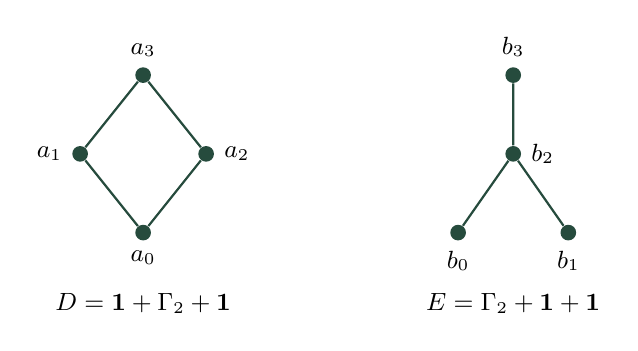
\begin{tikzpicture}[every node/.style={font=\small},
 dot/.style={circle,fill=forest,inner sep=2pt}]
 \node[dot,label=below:$a_0$] (a0) at (0,0) {};
 \node[dot,label=left:$a_1$] (a1) at (-.8,1) {};
 \node[dot,label=right:$a_2$] (a2) at (.8,1) {};
 \node[dot,label=above:$a_3$] (a3) at (0,2) {};
 \draw[forest,thick] (a0)--(a1)--(a3)--(a2)--(a0);
 \node at (0,-.9) {$D=\one+\anti2+\one$};
 \node[dot,label=below:$b_0$] (b0) at (4,0) {};
 \node[dot,label=below:$b_1$] (b1) at (5.4,0) {};
 \node[dot,label=right:$b_2$] (b2) at (4.7,1) {};
 \node[dot,label=above:$b_3$] (b3) at (4.7,2) {};
 \draw[forest,thick] (b0)--(b2)--(b1) (b2)--(b3);
 \node at (4.7,-.9) {$E=\anti2+\one+\one$};
\end{tikzpicture}
\caption{Hasse diagrams of the two factors. They have the same four
numerical invariants but different least-element flags.}
\label{fig:counterexample}
\end{figure}

Both have four points, height three, width two, and three incomparability
components. Consequently
\begin{equation}\label{eq:factor-tuples}
 (o(D),h(D),w(D),f(D))=(o(E),h(E),w(E),f(E))=(4,3,2,1).
\end{equation}
The factor $D$ has both endpoints. The factor $E$ has a greatest element
but no least element. Corollary~\ref{cor:finite-product} gives
\begin{equation}\label{eq:counterexample-values}
 f(D\times K)=8-3=5,
 \qquad
 f(E\times K)=8-2=6.
\end{equation}

\begin{theorem}[No formula from the four factor invariants]\label{thm:no-scalar}
There is no function $\Phi$ of eight ordinal arguments such that, for all
wpos $A,B$,
\[
 f(A\times B)=
 \Phi\bigl(o(A),h(A),w(A),f(A),o(B),h(B),w(B),f(B)\bigr).
\]
This fails already for finite factors of sizes four and two.
\end{theorem}
\begin{proof}
The two inputs to $\Phi$ obtained from $(D,K)$ and $(E,K)$ would be
identical by \eqref{eq:factor-tuples}. Their required outputs are different
by \eqref{eq:counterexample-values}.
\end{proof}

\subsection{Even the ordinary invariants of the products coincide}
The products both have maximal order type eight. Each has height four.
For an upper bound on height, use the rank functions
\[
 (0,1,1,2)\quad\text{on }D,
 \qquad (0,0,1,2)\quad\text{on }E,
\]
and add the $K$-coordinate, which is zero or one. Along a strict product
comparison this sum strictly increases, so a chain has at most four
points. A three-point chain in either base times $K$ contains a four-point
chain, giving equality.

Both product widths are three. In $D\times K$, an antichain is
\[
 \{(a_0,1),(a_1,0),(a_2,0)\},
\]
and a cover by three disjoint chains is
\[
\begin{aligned}
 &(a_0,0)<(a_1,0)<(a_3,0)<(a_3,1),\\
 &(a_0,1)<(a_1,1),\\
 &(a_2,0)<(a_2,1).
\end{aligned}
\]
In $E\times K$, an antichain is
\[
 \{(b_0,1),(b_1,1),(b_2,0)\},
\]
and a three-chain cover is
\[
\begin{aligned}
 &(b_0,0)<(b_2,0)<(b_3,0)<(b_3,1),\\
 &(b_0,1)<(b_2,1),\\
 &(b_1,0)<(b_1,1).
\end{aligned}
\]
These explicit certificates prove
\[
 (o,h,w)(D\times K)=(o,h,w)(E\times K)=(8,4,3).
\]
The friendly invariant detects information absent from these ordinary
product invariants as well as from the four factor invariants.

The multiset consequence is equally explicit:
\[
 w(M^r(D\times K))=\omega^5,
 \qquad
 w(M^r(E\times K))=\omega^6.
\]
Nothing in this example depends on numerical approximation. A complete
machine-readable certificate of legal friendly sequences is included in
the archive and summarized in Appendix~\ref{app:certificate}.

\subsection{How far apart two posets with the same elementary data can be}
Example~\ref{ex:three} can be pushed to the largest possible separation at
each cardinality.

\begin{proposition}[Maximal separation at fixed elementary invariants]\label{prop:separation}
For every $n\ge3$, the posets
\[
 L_n=\chain{n-2}+\anti2,
 \qquad
 R_n=\chain{n-1}\sqcup\chain1
\]
both have cardinality and maximal order type $n$, height $n-1$, and ordinary
width $2$, but
\[
 f(L_n)=1,\quad f(R_n)=n-1,
 \qquad
 w(M^r(L_n))=\omega,\quad w(M^r(R_n))=\omega^{n-1}.
\]
The gap $n-2$ is the largest possible between two non-chain $n$-element
posets.
\end{proposition}
\begin{proof}
In $L_n$ the chain summand contributes $n-2$ isolated vertices of the
incomparability graph and the top antichain contributes one further
component, so $c(L_n)=n-1$ and $f(L_n)=1$ by Theorem~\ref{thm:finite}. In
$R_n$ the isolated point is incomparable to all $n-1$ chain elements, so
$\Inc(R_n)$ is connected and $f(R_n)=n-1$. The height and width assertions
are immediate from the two constructions, and both maximal order types are
$n$ because both posets are finite with $n$ elements. Every non-chain finite
poset has friendly order type at least one by Lemma~\ref{lem:basic} and at
most $n-1$ by \eqref{eq:rough-bound}, so no larger gap is available.
\end{proof}

This separation and the product counterexample make different points.
Proposition~\ref{prop:separation} shows that $(|P|,o,h,w)$ leaves $f$ almost
entirely undetermined on a single poset. Theorem~\ref{thm:no-scalar} shows
something stronger and independent: even after $f$ itself is added to the
input data, the four-tuple still fails to determine $f$ of a product.

\section{Ordinal arithmetic and removal of finite tails}\label{sec:tails}

\subsection{Natural arithmetic versus ordinary arithmetic}
Every nonzero ordinal has a Cantor normal form
\[
 \alpha=\omega^{\xi_1}a_1+\cdots+\omega^{\xi_s}a_s,
 \qquad \xi_1>\cdots>\xi_s,\quad 0<a_i<\omega.
\]
The exponents are arbitrary ordinals. The natural sum $\alpha\oplus\beta$
adds coefficients of equal powers after aligning the exponents. The
natural product is obtained by distribution and the rule
\[
 (\omega^\xi a)\otimes(\omega^\eta b)
 =\omega^{\xi\oplus\eta}(ab).
\]
For example,
\begin{equation}\label{eq:cnf-example}
 (\omega+2)\otimes(\omega+3)=\omega^2+\omega\cdot5+6.
\end{equation}
Ordinary multiplication would give a different answer. Products of posets
use natural multiplication for maximal order type, by
\eqref{eq:mot-product}; ordinal sums of posets use ordinary ordinal
addition.

For a successor ordinal $\gamma+1$, define
\[
 \pred(\gamma+1)=\gamma.
\]
We call this the \emph{right predecessor}. We do not write a bare
``$\Theta-1$'' for it: ordinal subtraction conventions vary, and left
subtraction would not express the operation needed here. In Cantor normal
form a successor has a positive finite constant term. Its right
predecessor decreases that term by one and drops it if it becomes zero.

Every infinite ordinal has a unique decomposition
\begin{equation}\label{eq:finite-tail}
 \alpha=\lambda+m,
 \qquad \lambda\text{ a nonzero limit ordinal},\quad m<\omega.
\end{equation}
It is a successor exactly when $m>0$. In a natural product of finitely many
ordinals, the finite constant coefficient is the product of their finite
constant coefficients. In particular, a nonzero natural product has a
finite constant term zero if at least one factor is a nonzero limit.

\subsection{Removing finitely many points from a limit well-order}

\begin{lemma}\label{lem:finite-removal-ordinal}
If $\Lambda$ is a nonzero limit ordinal and $F\subseteq\Lambda$ is finite,
then the induced order on $\Lambda\setminus F$ has order type $\Lambda$.
\end{lemma}
\begin{proof}
It suffices to delete one point at a time. For a point at position $\beta$,
write
\[
 \Lambda=\beta+1+\tau,
\]
where $\tau$ is the order type of the interval strictly after that point.
Because $\Lambda$ is limit, this interval has no greatest point, so $\tau$
is a nonzero limit and in particular infinite. Hence $1+\tau=\tau$.
Deleting the point gives type $\beta+\tau=\beta+1+\tau=\Lambda$.
Iterate this argument for the finitely many deleted points.
\end{proof}

\begin{lemma}[Endpoint removal]\label{lem:endpoint-removal}
Let $P$ be an infinite wpo.
If $P$ has a least element $b$, then $o(P\setminus\{b\})=o(P)$.
If $P$ has a greatest element $g$, then
\[
 o(P)=o(P\setminus\{g\})+1.
\]
\end{lemma}
\begin{proof}
Every linear extension puts a least element first and a greatest element
last. Thus in the first case
$o(P)=1+o(P\setminus\{b\})$; the ordinal on the right after the $1$ is
infinite, so the initial $1$ is absorbed. In the second case the final $1$
is not absorbed, and the displayed equality follows. Attainment of the
maximal linearizations justifies both equalities directly.
\end{proof}

The asymmetry is essential. For an infinite product, a bottom point does
not cost a unit of maximal order type, while a top point does. For a finite
product, both endpoints cost a point. This is why the finite and infinite
formulas have different-looking corrections.

\subsection{An exact finite upper-tail lemma}

\begin{lemma}[Deleting the full finite upper tail]\label{lem:upper-tail}
Suppose $X$ is a wpo with
\[
 o(X)=\Lambda+N,
\]
where $\Lambda$ is a nonzero limit ordinal and $N$ is a positive integer.
Let $T\subseteq X$ be an upper set with exactly $N$ elements. Then
\begin{equation}\label{eq:core-mot}
 o(X\setminus T)=\Lambda.
\end{equation}
\end{lemma}
\begin{proof}
Put $Q=X\setminus T$. Choose a maximal linear extension of $X$ of type
$\Lambda+N$. Deleting $T$ leaves a well-order linear extension of $Q$.
Its restriction to the first $\Lambda$ positions has type $\Lambda$ after
finitely many deletions, by Lemma~\ref{lem:finite-removal-ordinal}. Hence
\[
 o(Q)\ge\Lambda.
\]

Since $T$ is an upper set, $Q$ is a downset. A maximal linear extension of
$Q$, followed by any linear extension of the finite poset $T$, is a linear
extension of $X$. There is no comparison from a point of $T$ upwards into
$Q$ that could prevent this concatenation. Consequently
\[
 o(Q)+N\le\Lambda+N.
\]
If $o(Q)>\Lambda$, then $o(Q)\ge\Lambda+1$ and
\[
 o(Q)+N\ge\Lambda+(N+1)>\Lambda+N,
\]
a contradiction. Therefore $o(Q)\le\Lambda$, proving equality.
\end{proof}

The equality between $|T|$ and the final finite coefficient $N$ is part of
the hypothesis. The lemma does not assert that deleting an arbitrary
finite set always removes exactly the finite tail of maximal order type.
Its upper-set hypothesis also has a precise role: it makes the
concatenated extension of $Q$ and $T$ valid.

\section{Products of infinite ordinals with a finite poset}\label{sec:mixed}

\subsection{Statement of the main transfinite theorem}

\begin{theorem}[Mixed ordinal--finite products]\label{thm:mixed}
Let $r\ge1$, let $\alpha_1,\ldots,\alpha_r$ be infinite ordinals, and let
$B$ be a nonempty finite poset. Assume
\[
 r\ge2\quad\text{or}\quad |B|\ge2.
\]
Define
\[
 P=\alpha_1\times\cdots\times\alpha_r\times B,
 \qquad
 \Theta=\alpha_1\otimes\cdots\otimes\alpha_r\otimes |B|.
\]
Then
\begin{equation}\label{eq:mixed}
 \boxed{
 f(P)=
 \begin{cases}
  \pred(\Theta),&\text{all $\alpha_i$ are successors and $B$ has a greatest element},\\[2pt]
  \Theta,&\text{otherwise}.
 \end{cases}}
\end{equation}
In the omitted case $r=1$ and $|B|=1$, the poset is a chain and $f(P)=0$.
\end{theorem}

We divide the proof into the limit case, an exact identification of the
infinite core, and a finite friendly deletion of the upper corner. These
are separate tasks: a maximal-order-type computation alone does not
supply the required friendly witnesses.

\subsection{At least one limit factor}
Suppose some $\alpha_i$ is a limit ordinal. The natural-product formula
gives $o(P)=\Theta$, and $\Theta$ is a nonzero limit because its constant
Cantor coefficient is zero. There is no greatest element of $P$.

The nondegeneracy assumption allows application of
Theorem~\ref{thm:product-components}. Thus the only possible friendless
point is the least point, if $B$ has one. Lemma~\ref{lem:endpoint-removal}
shows that its deletion does not change the infinite maximal order type.
Hence
\[
 o(\str(P))=o(P)=\Theta.
\]
Published limit saturation, Theorem~\ref{thm:imported-limit}, now gives
$f(P)=\Theta$, as required. This argument covers the known two-limit
special case and also limit factors paired with finite or successor
factors in the present family.

\subsection{All factors have finite successor tails}
From now on, assume that every $\alpha_i$ is a successor. Write uniquely
\[
 \alpha_i=\lambda_i+m_i,
 \qquad \lambda_i\text{ a nonzero limit},\quad 1\le m_i<\omega.
\]
The \emph{finite upper corner} and its complement are
\begin{equation}\label{eq:corner}
 T=\prod_{i=1}^r[\lambda_i,\alpha_i)\times B,
 \qquad Q=P\setminus T,
 \qquad N=|T|=|B|\prod_{i=1}^r m_i.
\end{equation}
The set $T$ is upper. The constant Cantor coefficient of $\Theta$ is $N$,
so there is a nonzero limit $\Lambda$ such that
\begin{equation}\label{eq:theta-tail}
 \Theta=\Lambda+N.
\end{equation}
Lemma~\ref{lem:upper-tail} proves $o(Q)=\Lambda$.

We next prove that $Q$ retains enough incomparability to have friendly
order type $\Lambda$. This is not automatic for an arbitrary downset of a
product.

\begin{lemma}[The core has no new friendless points]\label{lem:core-stripped}
Every point of $Q$ other than a possible least point of $P$ has an
incomparable friend in $Q$. Consequently
\[
 o(\str(Q))=\Lambda,\qquad f(Q)=\Lambda.
\]
\end{lemma}
\begin{proof}
Let $x=(x_1,\ldots,x_r,b)\in Q$ be different from a possible least point.
It is not a greatest point of $P$, since any such point belongs to $T$.
Theorem~\ref{thm:product-components} provides $y\in P$ with $x\perp y$.
If $y\in Q$, we are done.

Otherwise $y\in T$. As $x\in Q$, choose $i$ with $x_i<\lambda_i$.
Replace just the $i$-th coordinate of $y$ by $x_i+1$ and call the resulting
point $y'$. The limit property gives
\[
 x_i<x_i+1<\lambda_i,
\]
so $y'\in Q$ and $y'\not\le x$. Also $x\not\le y$ was witnessed in a
coordinate other than $i$, or in $B$: the original $i$-th coordinate of
$y$ was at least $\lambda_i>x_i$ and therefore could not have caused
$x\not\le y$. That witness is unchanged. Hence $x\not\le y'$ and
$x\perp y'$.

This shows that $\str(Q)$ is either $Q$ or $Q$ with its least point
removed. Since $o(Q)=\Lambda$ is infinite, endpoint removal leaves the
same maximal order type. Applying Theorem~\ref{thm:imported-limit} to $Q$
gives $f(Q)=\Lambda$.
\end{proof}

\subsection{A finite factor with no greatest element}
Assume $B$ has no greatest element. For every $b\in B$ there is a
$c\in B$ with $c\not\le b$, because otherwise $b$ would be greatest.
For a point $x=(x_1,\ldots,x_r,b)\in T$, the point
\[
 q_x=(0,\ldots,0,c)\in Q
\]
is incomparable with $x$: the $B$-coordinate prevents $q_x\le x$, while
$x_1\ge\lambda_1>0$ prevents $x\le q_x$.

Select all $N$ points of $T$ in a reverse linear extension of its induced
order. At each stage the selected point is maximal among the remaining
points of $T$. Its upper set is contained in $T$, so the move deletes
only itself. The witness $q_x$ lies in $Q$, which none of these moves
alters. Thus all $N$ selections are legal and leave exactly $Q$.
By Lemmas~\ref{lem:basic} and \ref{lem:core-stripped},
\[
 f(P)\ge f(Q)+N=\Lambda+N=\Theta.
\]
The reverse inequality follows from $f(P)\le o(P)=\Theta$. This proves
the second case of \eqref{eq:mixed} when all ordinal factors are successors
but $B$ has no greatest point.

\subsection{A greatest point: the sharp upper bound}
Now assume $B$ has greatest element $b^*$. Let $t_i$ be the greatest point
of $\alpha_i$, so $t_i+1=\alpha_i$. The product has greatest point
\[
 g=(t_1,\ldots,t_r,b^*).
\]
By Theorem~\ref{thm:product-components}, stripping removes exactly $g$ and,
possibly, the least point. Applying Lemma~\ref{lem:endpoint-removal} gives
\[
 o(\str(P))=\Lambda+(N-1)=\pred(\Theta).
\]
Therefore
\begin{equation}\label{eq:mixed-top-upper}
 f(P)\le\Lambda+(N-1).
\end{equation}

If $N=1$, the lower bound $f(P)\ge f(Q)=\Lambda$ already gives equality.
No legal corner move is claimed in this case. The unique corner point is
the greatest point and has no friend.

\subsection{A greatest point: deleting the corner in $N-1$ moves}
Assume $N>1$. Define the top edge
\[
 E=\{(\lambda_1+j,t_2,\ldots,t_r,b^*):0\le j<m_1\}\subseteq T.
\]
The point $g$ is the last point of this edge. We will select every point
of $T$ except $g$, but do so in an order that allows $g$ to disappear
incidentally rather than being selected illegally.

\subsubsection{Phase I: the top edge below its greatest point}
Select the points of $E\setminus\{g\}$ in descending order of their
first coordinate. The first selection, when this phase is nonempty,
removes itself and $g$; each later selection in this phase removes only
itself. Indeed, all coordinates except the first are already greatest,
so its upper set lies on $E$.

The following friend survives throughout the phase. If $r\ge2$, take
\[
 y=(t_1,0,t_3,\ldots,t_r,b^*)\in Q.
\]
For every selected $x\in E\setminus\{g\}$, its first coordinate is
strictly below $t_1$, while its second coordinate is $t_2>0$. Thus
$x\perp y$, and the second coordinate also keeps $y$ out of all the upper
sets removed in this phase.

If $r=1$, our assumption forces $|B|\ge2$. Choose $b_0\ne b^*$, so
$b_0<b^*$. The point
\[
 y=(t_1,b_0)\in T\setminus E
\]
is incomparable with each selected top-edge point and survives every
Phase I deletion. This separate argument is why the single-chain
exception cannot simply be ignored.

\subsubsection{Phase II: the rest of the corner}
Select $T\setminus E$ in any reverse linear extension. A single permanent
friend works for every selection:
\[
 q=(0,t_2,\ldots,t_r,b^*)\in Q.
\]
For $x\in T\setminus E$, its first coordinate exceeds zero, so
$x\not\le q$. Since $x$ is not on $E$, some other ordinal coordinate is
strictly below its top value, or its $B$-coordinate is strictly below
$b^*$. This prevents $q\le x$. Hence $x\perp q$.

All upper sets of selected points remain inside $T$, so $q$ survives.
The reverse linear extension makes each selected point maximal among the
remaining points of $T\setminus E$. All points of $E\setminus\{g\}$
have already gone. If Phase I was empty, the first Phase II selection may
also delete $g$; otherwise $g$ is already absent. No unselected point of
$T\setminus E$ is deleted prematurely.

There are
\[
 (|E|-1)+|T\setminus E|=N-1
\]
selected points. If Phase I is empty and $N>1$, then $T\setminus E$ is
nonempty, so $g$ is indeed deleted in Phase II. The final residual is
exactly $Q$. It follows that
\[
 f(P)\ge f(Q)+(N-1)=\Lambda+(N-1).
\]
Together with \eqref{eq:mixed-top-upper}, this proves equality and completes
the proof of Theorem~\ref{thm:mixed}.
\hfill$\square$

\subsection{Why the method is genuinely transfinite}
The finite corner contributes a finite number of successors \emph{after}
the rank of an infinite residual. In schematic form the argument is
\[
 \underbrace{f(Q)}_{\Lambda}
 \quad+\quad
 \underbrace{\text{number of certified corner moves}}_{N\text{ or }N-1}.
\]
This is an ordinal-rank argument using the residual equation, not a claim
that one can perform $\Lambda$ moves before entering the corner. Every
actual friendly bad sequence is finite. Transfinite complexity is encoded
by the branching and nested ranks of its tree.

The core calculation and the corner strategy also have logically distinct
roles. The maximal-linearization theorem and limit saturation establish
$f(Q)=\Lambda$. The explicit witnesses establish the successor correction.
Neither part can be replaced by a numerical extrapolation from finite
grids.

\section{Complete classification of ordinal boxes}\label{sec:boxes}

\subsection{All degeneracies included}

\begin{theorem}[Finite products of ordinals]\label{thm:boxes}
Let
\[
 P=\prod_{i=1}^d\alpha_i
\]
with componentwise order, where the $\alpha_i$ are ordinals and $d<\omega$.
The empty product is a singleton. Then the following rules determine
$f(P)$ completely.
\begin{enumerate}[label=(\arabic*)]
\item If some factor is zero, then $f(P)=0$.
\item Otherwise discard all factors equal to one. If at most one factor
remains, then $f(P)=0$.
\item If at least two factors remain and they are all finite, then
\[
 f(P)=\prod_i\alpha_i-3.
\]
\item If at least two factors remain and at least one is infinite, put
$\Theta=\bigotimes_i\alpha_i$. Then
\[
 f(P)=
 \begin{cases}
  \Theta,&\text{some factor is a limit ordinal},\\
  \pred(\Theta),&\text{every factor is a successor ordinal}.
 \end{cases}
\]
\end{enumerate}
\end{theorem}
\begin{proof}
A zero factor makes the product empty, and singleton factors do not alter
its order type. With at most one non-singleton factor the result is a
chain. If every remaining factor is finite, the product has both endpoints
and at least two non-singleton factors, so Corollary~\ref{cor:finite-product}
gives its cardinality minus three.

In the infinite case, group the finite factors into a finite poset $B$;
if there are none, let $B$ be a singleton. It has a greatest element. The
nondegeneracy assumption of Theorem~\ref{thm:mixed} holds because at least
two non-singleton factors remain in total. That theorem gives exactly the
last two cases. Natural-product associativity identifies its $\Theta$
with the displayed natural product of all original factors.
\end{proof}

\subsection{Worked calculations}
The following examples use ordinary addition in the displayed Cantor
normal forms. Multiplications by finite coefficients are written on the
right.

\begin{table}[ht]
\centering\small
\renewcommand{\arraystretch}{1.3}
\begin{tabularx}{\textwidth}{@{}Y Y Y@{}}
\toprule
\textbf{Poset $P$} & \textbf{Maximal order type $o(P)$} & \textbf{Friendly order type $f(P)$}\\
\midrule
$\omega\times3$ & $\omega\cdot3$ & $\omega\cdot3$\\
$(\omega+2)\times3$ & $\omega\cdot3+6$ & $\omega\cdot3+5$\\
$(\omega+1)\times(\omega+1)$ & $\omega^2+\omega\cdot2+1$ & $\omega^2+\omega\cdot2$\\
$(\omega+2)\times(\omega+3)$ & $\omega^2+\omega\cdot5+6$ & $\omega^2+\omega\cdot5+5$\\
$(\omega+1)\times\anti2$ & $\omega\cdot2+2$ & $\omega\cdot2+2$\\
$(\omega+1)\times D$ & $\omega\cdot4+4$ & $\omega\cdot4+3$\\
\bottomrule
\end{tabularx}
\caption{Exact values. The antichain example uses the mixed-product
theorem rather than the ordinal-box corollary: its finite factor has no
greatest element.}
\label{tab:examples}
\end{table}

For an example with three nonconstant terms, distribution gives
\[
 (\omega^2+3)\otimes(\omega+2)
 =\omega^3+\omega^2\cdot2+\omega\cdot3+6.
\]
Both factors are successors, so
\[
 f\bigl((\omega^2+3)\times(\omega+2)\bigr)
 =\omega^3+\omega^2\cdot2+\omega\cdot3+5.
\]
For an example requiring hereditary exponents,
\begin{align*}
 &(\omega^\omega+\omega+4)\otimes(\omega^2+2)\\
 &\qquad=\omega^{\omega+2}+\omega^\omega\cdot2
       +\omega^3+\omega^2\cdot4+\omega\cdot2+8.
\end{align*}
The friendly order type of the corresponding product is the same expression
with final coefficient $7$ instead of $8$. Here the leading exponent
arises from the natural sum $\omega\oplus2=\omega+2$.

There is no countability restriction. For instance,
\[
 f\bigl((\omega_1+1)\times2\bigr)=\omega_1\cdot2+1.
\]
One can calculate the natural product using
$\omega_1=\omega^{\omega_1}$: all powers $\omega^\xi$ for $\xi<\omega_1$
are countable and their supremum is $\omega_1$. Thus its Cantor form is a
single monomial, and natural multiplication by two doubles the coefficient.
This example is a mathematical consequence of the theorem, not an output
of the below-$\varepsilon_0$ software.

\subsection{Finite-grid approximation is not a proof}
For finite $n\ge2$, the finite product formula gives
\[
 f(n\times2)=2n-3.
\]
The supremum of these values is $\omega$, whereas
\[
 f(\omega\times2)=\omega\cdot2.
\]
Thus even an exhaustive list of all finite rectangles of this shape would
not determine the friendly order type of their union by taking numerical
suprema. A friendly-tree node can have arbitrarily high residual rank
without there being a branch of corresponding infinite length. The
finite checks in the archive are deliberately not advertised as a
verification of the transfinite theorem.

This caution is about \emph{method}: numerical suprema of finite instances
do not compute a transfinite rank. It should not be confused with the
separate, mathematical obstruction of
Proposition~\ref{prop:graph-obstruction} below, which says that on infinite
wpos the isomorphism type of the incomparability graph no longer determines
the invariant at all, however it is computed. The first is a warning about
extrapolating from data; the second is a theorem about what the data could
possibly contain.

\section{Ordinal sums and a compositional class}\label{sec:sums}

\subsection{The sum rule}
The binary identity below is already known
\cite[Theorem~5.4.8(1)]{VialardThesis}. We give a proof to fix the direction
of ordinal addition and then record its transfinite extension.

\begin{proposition}\label{prop:binary-sum}
For wpos $A,B$,
\[
 f(A+B)=f(A)+f(B).
\]
\end{proposition}
\begin{proof}
Use transfinite induction on $f(B)$, simultaneously for all $A$. A
friendly first move in $A$ must have its friend in $A$ and deletes all of
$B$. These first moves contribute a supremum of $f(A)$ to the residual
rank formula. A friendly first move $b$ in $B$ has its friend in $B$ and
leaves $A+\res B b$. Since
$f(\res B b)+1\le f(B)$, induction applies to this residual and gives
\[
 f(A+\res B b)+1
   =f(A)+f(\res B b)+1.
\]
If $f(B)=0$, there are no such moves, giving the result directly. If
$f(B)>0$, take the supremum over them. Ordinary ordinal addition is
continuous in its right argument at limits, and a supremum which is a
successor is attained. Consequently this supremum is
\[
 f(A)+\sup_b\bigl(f(\res B b)+1\bigr)=f(A)+f(B).
\]
It dominates the contribution $f(A)$ from first moves in $A$. This proves
the formula in all cases, including empty factors.
\end{proof}

The induction may equally be run on the rank of $\Bad(B)$ rather than on
$f(B)$: a residual $\res B b$ has strictly smaller bad-sequence rank, and
nothing else in the argument changes. This is a choice of induction measure,
not a different proof.

The finite case of the ordinal sum has a companion for the disjoint union,
which behaves in the opposite way.

\begin{corollary}[Finite sums and disjoint unions]\label{cor:finite-sums}
For finite posets $A,B$,
\[
 f(A+B)=f(A)+f(B).
\]
If moreover $A$ and $B$ are both nonempty, then
\[
 f(A\sqcup B)=|A|+|B|-1.
\]
\end{corollary}
\begin{proof}
The first identity is the finite case of
Proposition~\ref{prop:binary-sum}; equivalently, the incomparability graph
of an ordinal sum is the disjoint union of the two incomparability graphs,
so vertex and component counts both add and
Theorem~\ref{thm:finite} applies. In the poset disjoint union, by contrast,
every vertex of $A$ is incomparable to every vertex of $B$, so the resulting
incomparability graph is connected when both parts are nonempty. Hence
$c(A\sqcup B)=1$, and Theorem~\ref{thm:finite} gives $|A|+|B|-1$.
\end{proof}

The disjoint-union identity is consistent with the published finite
formulas and is not claimed here as a new special case; what the component
theorem adds is the common structural explanation of both identities.

\begin{theorem}[Well-ordered sums]\label{thm:ordinal-sum}
Let $(P_i)_{i<\eta}$ be wpos indexed by an ordinal. Their ordinal sum is a
wpo, and
\begin{equation}\label{eq:ordinal-sum}
 f\left(\sum_{i<\eta}P_i\right)=\sum_{i<\eta}f(P_i),
\end{equation}
where the right-hand sum is the ordinary transfinite ordinal sum.
\end{theorem}
\begin{proof}
An infinite bad sequence in the sum cannot move to a strictly higher
block. Its block indices would therefore be nonincreasing and eventually
constant, since ordinals have no infinite strict descent. Its tail would
be an infinite bad sequence within one block, a contradiction.

The friendly formula follows by transfinite induction on $\eta$.
The successor step is Proposition~\ref{prop:binary-sum}. Suppose $\eta$
is limit. Each initial subsum embeds into the whole sum, so monotonicity
gives the lower bound by the supremum of their friendly order types.
For the upper bound, a first move in block $P_j$ deletes all higher blocks.
It is legal precisely when it is legal in the subsum through $P_j$, since
its friend must lie in the same block. Its residual and rank contribution
are therefore the same as in that initial subsum. Taking the supremum
of all first-move contributions gives no more than the supremum of the
friendly order types of the initial subsums. This equals the transfinite
sum on the right of \eqref{eq:ordinal-sum}.
\end{proof}

For finite blocks the formula becomes especially concrete:
\begin{equation}\label{eq:finite-blocks}
 f\left(\sum_{i<\eta}P_i\right)
 =\sum_{i<\eta}\bigl(|P_i|-c(P_i)\bigr).
\end{equation}
The finite subtraction takes place \emph{inside each summand}; the outer sum
is ordinal addition in the displayed order, not natural addition and not
cardinal addition. Consequently a final finite block can survive in the
answer where the same block placed at the beginning would be absorbed.

\begin{corollary}[Arbitrary wpo with finite components]\label{cor:finite-components}
Let $P$ be a wpo all of whose incomparability components are finite, and let
$(C_\xi)_{\xi<\eta}$ be those components in their canonical well-ordered
sequence. Then
\begin{equation}\label{eq:finite-components-infinite}
 f(P)=\sum_{\xi<\eta}\bigl(|C_\xi|-1\bigr).
\end{equation}
\end{corollary}
\begin{proof}
Lemma~\ref{lem:ordered-components} exhibits $P$ as the well-ordered sum of
its components, which is a well-order by the remark following that lemma.
Each block is finite with connected incomparability graph, so
$|C_\xi|-c(C_\xi)=|C_\xi|-1$. Apply \eqref{eq:finite-blocks}.
\end{proof}

\subsection{Explicit transfinite values}
Write $H=\sum_{n<\omega}\anti2$, an $\omega$-indexed ordinal sum of
two-element antichains. Then
\[
 f(H)=\omega,\qquad w(M^r(H))=\omega^\omega .
\]
For $k<\omega$,
\[
 f(H+\anti{k+1})=\omega+k,
 \qquad
 w\bigl(M^r(H+\anti{k+1})\bigr)=\omega^{\omega+k},
\]
so the final finite block is not absorbed. Likewise
$\sum_{\xi<\omega^2}\anti2$ has friendly order type $\omega^2$. Inserting
arbitrary chain blocks anywhere in such a sum adds nothing, since their
contribution is zero: for instance, appending a chain of type $\omega$ to
$H$ gives $f(H+\omega)=\omega+0=\omega$, whereas
$o(H+\omega)=\omega\cdot2$. A long comparable tail can change maximal
order type without creating any new friendly moves.

\begin{corollary}[Every ordinal, at ordinary width two]\label{cor:all-ordinals}
For every ordinal $\alpha$ put
\[
 P_\alpha=\sum_{\xi<\alpha}\anti2 .
\]
Then $f(P_\alpha)=\alpha$ and $w(M^r(P_\alpha))=\omega^\alpha$. For
$\alpha>0$ the ordinary maximum antichain size of $P_\alpha$ is exactly two.
\end{corollary}
\begin{proof}
Every two-element antichain contributes $2-1=1$ to
\eqref{eq:ordinal-sum}, and the transfinite sum of $\alpha$ copies of $1$ is
$\alpha$. An antichain of $P_\alpha$ cannot meet two different blocks, since
distinct blocks are completely comparable, and each nonempty block has an
antichain of size two. Apply \eqref{eq:multiset} for the width.
\end{proof}

\begin{proposition}[The infinite graph-only obstruction]\label{prop:graph-obstruction}
On infinite wpos, the friendly order type is not determined by the
isomorphism type of the incomparability graph, even when every component is
finite. Indeed, for all countably infinite ordinals $\alpha$ the graphs
$\Inc(P_\alpha)$ are pairwise isomorphic, while $f(P_\alpha)=\alpha$.
\end{proposition}
\begin{proof}
For countably infinite $\alpha$, the graph $\Inc(P_\alpha)$ is a disjoint
union of countably infinitely many isolated edges, one per block, and any
bijection between two such block index sets induces a graph isomorphism.
The friendly order types are given by Corollary~\ref{cor:all-ordinals} and
need not coincide: $\omega$ and $\omega+1$ already differ.
\end{proof}

So the finite graphic-rank reading of Corollary~\ref{cor:graphic} is exact
but does not extend unchanged to infinite graphs. What the infinite case
additionally requires is the \emph{order} of the components, which carries
indispensable ordinal information that the abstract graph discards. Note
what is and is not claimed: these transfinite values are consequences of
the sum law applied to blocks we control completely. They are not a claim
that the general connected infinite case has been solved.

\subsection{A usable structural language}
The results provide an exact evaluator on descriptions built from finite
posets, finite ordinal boxes, finite disjoint unions and lexicographic
substitutions with nonempty finite fibers
(Corollary~\ref{cor:finite-sums} and Theorem~\ref{thm:substitution}), the
mixed products of Theorem~\ref{thm:mixed}, and well-ordered sums of already
evaluated expressions. On the finite part the evaluator needs no recursion
at all: by Theorem~\ref{thm:finite} it reads the answer off the
incomparability graph. A product node in this language must satisfy the
proved hypotheses. An arbitrary product of two previously generated
expressions is not automatically covered.

This distinction prevents an erroneous overstatement. Closure under
ordinal sums, together with some exact product rules, is not closure under
all Cartesian products. The counterexample in
Theorem~\ref{thm:no-scalar} shows that a general evaluator cannot merely
store the tuple $(o,h,w,f)$ and discard the rest of the structure.

\section{Enumeration and a bivariate generating function}\label{sec:enumeration}

The component decomposition \eqref{eq:component-sum} is rigid enough to
count finite posets by their friendly rank exactly, not merely to tabulate
them.

Call a poset on $\{0,1,\ldots,n-1\}$ \emph{naturally labelled} when
$i<_Pj$ implies $i<j$ as integers. Let $a_n$ count such posets, with
$a_0=1$, and let $b_n$ count those of them whose incomparability graph is
connected, for $n\ge1$. These are neither counts of unlabelled posets nor
counts of all labelled posets: every isomorphism type has at least one
natural labelling, but it usually has many. Put
\[
 \gfA(z)=\sum_{n\ge0}a_nz^n,
 \qquad
 \gfB(z)=\sum_{n\ge1}b_nz^n.
\]
In this section only, the sans-serif letters $\gfA$ and $\gfB$ denote formal
power series, not posets; no analytic convergence is asserted. Let $a_{n,k}$
count naturally labelled $n$-element posets with friendly order type $k$.

\begin{theorem}[Distribution by component rank]\label{thm:gf}
One has
\begin{equation}\label{eq:gf-univariate}
 \gfA(z)=\frac{1}{1-\gfB(z)},
 \qquad
 b_n=a_n-\sum_{i=1}^{n-1}b_i\,a_{n-i},
\end{equation}
and the bivariate distribution is
\begin{equation}\label{eq:gf}
 \boxed{\sum_{n,k\ge0}a_{n,k}z^nu^k
 =\frac{1}{1-\sum_{m\ge1}b_mz^mu^{m-1}}.}
\end{equation}
For $n\ge1$ and $0\le k\le n-1$,
\begin{equation}\label{eq:gf-coefficient}
 a_{n,k}=[z^n]\,\gfB(z)^{\,n-k}.
\end{equation}
\end{theorem}
\begin{proof}
In a natural labelling, if $C<D$ are incomparability components then every
label in $C$ is smaller than every label in $D$, by
Lemma~\ref{lem:ordered-components}. Components therefore occupy consecutive
intervals of labels in their canonical order, and
\eqref{eq:component-sum} becomes a unique ordered list of nonempty naturally
labelled posets with connected incomparability graph. Conversely,
concatenating any such list by ordinal sum yields a naturally labelled poset
with exactly those components. Summing over ordered lists gives
$1+\gfB+\gfB^2+\cdots$, which is the first identity; extracting coefficients
gives the recurrence.

A component of size $m$ contributes $m-1$ to the friendly order type by
Theorem~\ref{thm:finite}, so weighting it by $z^mu^{m-1}$ proves
\eqref{eq:gf}. A poset of size $n$ and friendly order type $k$ has exactly
$n-k$ components, so extracting from lists of that length gives
\eqref{eq:gf-coefficient}.
\end{proof}

The exhaustive enumeration described in Section~\ref{sec:computation} gives
\[
 (a_0,\ldots,a_7)=(1,1,2,7,40,357,4824,96428)
\]
and, through \eqref{eq:gf-univariate},
\[
 (b_1,\ldots,b_7)=(1,1,4,27,275,4070,86278).
\]
These values are outputs of the included exact enumeration, recomputed for
this report, not numbers taken from a database without verification.

\begin{corollary}[Fixed-rank counting polynomials]\label{cor:polynomial}
For fixed $k\ge0$ and $n\ge k+1$,
\begin{equation}\label{eq:fixed-rank}
 a_{n,k}=
 \sum_{\substack{m_1,\ldots,m_k\ge0\\ \sum_{j=1}^kjm_j=k}}
 \frac{(n-k)_{\underline r}}{\prod_{j=1}^km_j!}
 \prod_{j=1}^kb_{j+1}^{\,m_j},
 \qquad r=\sum_{j=1}^km_j,
\end{equation}
where $(x)_{\underline r}=x(x-1)\cdots(x-r+1)$ and empty products are $1$.
As a function of $n$ this is a polynomial of degree $k$ with leading
coefficient $1/k!$.
\end{corollary}
\begin{proof}
There are $n-k$ component positions. Let $m_j$ record how many components
have size $j+1$; their total rank contribution is $\sum_jjm_j=k$, and all
remaining components are singletons. Choose and order the $r$ non-singleton
positions in $(n-k)_{\underline r}/\prod_jm_j!$ ways, then choose the
connected structure on each. The degree is at most $r\le k$, and degree $k$
occurs only when $m_1=k$; since $b_2=1$, that term is $\binom{n-k}{k}$,
whose leading coefficient is $1/k!$.
\end{proof}

For example, within their indicated ranges of $n$,
\begin{align*}
 a_{n,0}&=1,\\
 a_{n,1}&=n-1,\\
 a_{n,2}&=4(n-2)+\binom{n-2}{2}=\frac{(n-2)(n+5)}{2},\\
 a_{n,3}&=27(n-3)+4(n-3)(n-4)+\binom{n-3}{3}.
\end{align*}
These give a combinatorial explanation of the initial columns of
Table~\ref{tab:finite-tests}, rather than only an empirical pattern in the
data.

\section{Algorithms, experiments, and reproducibility}\label{sec:computation}

\subsection{Two independent finite engines}
Both engines represent a finite partial order by its inclusive principal
upper sets as integer bit masks, and both validate reflexivity,
antisymmetry, transitivity and mask bounds; the relation-based constructors
first take a transitive closure and reject cycles.

The module \texttt{code/friendly.py} carries the constructions of
Sections~\ref{sec:finite}--\ref{sec:subsets}: the protected-root non-cut
step of Lemma~\ref{lem:noncut}, the optimal certificate with its
spanning-forest roots, the certificate verifier, lexicographic substitution,
order duals, and the efficient ideal-based enumeration of naturally labelled
orders. The module \texttt{code/finite\_posets.py} is a separate
implementation, with its own enumerator, its own residual dynamic program,
its own search-based constructive-certificate routine, and the
height, width, cover and product machinery used for the counterexample of
Section~\ref{sec:counterexample}. Agreement between them is agreement
between two implementations, not a routine calling itself.

The direct algorithm, present in both, implements the defining residual
equation:
\begin{lstlisting}[language=Python]
def rank(mask):
    best = 0
    for x in elements(mask):
        if incomparable[x] & mask:
            after = mask & ~upper[x]
            best = max(best, 1 + rank(after))
    return best
\end{lstlisting}
Memoization makes each residual state run at most once. This algorithm
\emph{does not call} the component formula and does not use
Lemma~\ref{lem:noncut}, so comparison against it is not a test of the
formula against itself. It also reconstructs an optimal
sequence and supplies an actual friend at every move, along with the
residual before and after the move.

A second evaluator builds the incomparability graph, counts its components,
and returns $n-c(P)$. On an explicit comparison matrix this needs
$O(n^2)$ operations: forming the graph and searching its components are
enough, and the multiset width is then reported symbolically as $\omega^k$
with no attempt to enumerate the infinite multiset order. If only covering
or generating relations are supplied, a transitive closure comes first, and
a naive transitivity check alone costs $O(n^3)$; the quadratic claim is for
evaluation after a valid comparison matrix is given, not for every input
representation. The direct rank algorithm has up to $2^n$ residual masks,
so it is an exponential reference checker rather than the intended efficient
method. Under unit-cost mask operations its bound is $O(n2^n)$ subset
transitions.

For the constructive witness there are two routines, and their costs differ
because their strategies differ. The routine in \texttt{code/friendly.py}
implements Lemma~\ref{lem:noncut} directly: one non-cut step selects a
maximal vertex distinct from the protected root, computes the components
after its deletion, and, if that vertex was a cut vertex, takes a maximal
element of the last new component exactly as in the proof. Such a step costs
$O(n^2)$ elementary operations on a comparison matrix, and there are at most
$n-1$ steps, so a full witness with its at most $n-1$ choice--friend pairs
is constructed in $O(n^3)$. The routine in
\texttt{code/finite\_posets.py} instead searches the maximal vertices and
tests each candidate deletion, which is a conservative $O(n^4)$; it is kept
because it is an independent implementation, not because it is the best
bound available. Both are logically independent of the residual dynamic
program. All these bounds are stated in the elementary-operation model: the
Python implementations use arbitrary-precision integer bit sets, and we do
not pretend that long machine integers have unit cost.

The verifier checks every emitted move against the original relation, not
just the final length: it simulates the residuals, confirms that each named
choice and friend is still present and incomparable, checks by union--find
that the witness edges are acyclic, and checks that they span each original
incomparability component with one declared root apiece. That establishes
legality and confirms the forest certificate of
Proposition~\ref{prop:forest}; optimality is then certified by comparing the
sequence length with the component upper bound of
Corollary~\ref{cor:upper}.

\subsection{Exhaustive finite checks}
All partial orders compatible with the fixed linear extension
$0<1<\cdots<n-1$ were generated for $0\le n\le7$. These are
\emph{naturally labelled} posets. They are not all label permutations and
are not quotiented by isomorphism. Every finite isomorphism class of the
relevant size has at least one representative in this enumeration, generally
several. To pass from size $n-1$ to size $n$, the strict predecessor set of
the new largest label is chosen among the order ideals of the previous
order: every such ideal gives a valid natural order, and every natural order
arises exactly once this way.

\begin{table}[ht]
\centering\small
\begin{tabular}{@{}rrrrrrrrr@{}}
\toprule
$n$ & Total & $f=0$ & $f=1$ & $f=2$ & $f=3$ & $f=4$ & $f=5$ & $f=6$\\
\midrule
0 & 1 & 1 & -- & -- & -- & -- & -- & --\\
1 & 1 & 1 & -- & -- & -- & -- & -- & --\\
2 & 2 & 1 & 1 & -- & -- & -- & -- & --\\
3 & 7 & 1 & 2 & 4 & -- & -- & -- & --\\
4 & 40 & 1 & 3 & 9 & 27 & -- & -- & --\\
5 & 357 & 1 & 4 & 15 & 62 & 275 & -- & --\\
6 & 4,824 & 1 & 5 & 22 & 106 & 620 & 4,070 & --\\
7 & 96,428 & 1 & 6 & 30 & 160 & 1,047 & 8,906 & 86,278\\
\bottomrule
\end{tabular}
\caption{Exhaustive naturally labelled orders by friendly rank, totalling
$101{,}660$ orders including the empty poset. For each order the test
compares the direct residual rank with $n-c(P)$, repeats the direct
recursion on the dual order, and constructs and simulates an optimal
certificate with its spanning forest. The machine-readable form is
\texttt{data/rank\_distribution.csv}.}
\label{tab:finite-tests}
\end{table}

Every comparison passed. The maximal non-cut conclusion of
Lemma~\ref{lem:noncut} was additionally checked at the root of every
connected case of size at least two, which is $90{,}655$ explicit checks.
Separately, the independent \texttt{FinitePoset} engine re-derived the same
values, together with its own constructive certificates, on all $5{,}231$
nonempty orders through size six and on the empty poset; this is a
cross-implementation check over a smaller range, not a second
exhaustive-enumeration figure.

The composition laws were tested as follows.
\begin{itemize}
\item \emph{Products.} All $2{,}601$ ordered pairs of naturally labelled
factors of sizes zero through four, comparing the graph count and the
independent residual recursion with \eqref{eq:finite-product}, including the
degenerate empty and singleton factors. Product supports reach sixteen
elements. On the $2{,}401$ of those pairs with both factors of size at least
two, the unique non-endpoint incomparability component asserted by
Theorem~\ref{thm:product-components} was also checked.
\item \emph{Substitutions.} Every natural base of size at most four, with
each fiber independently chosen from a singleton, a two-element chain, a
two-element antichain and a three-element chain: $10{,}725$ heterogeneous
substitutions, each checked against the direct residual recursion and
against \eqref{eq:substitution}.
\item \emph{Maximum friendly subsets.} Through support size five,
$2{,}365$ candidate subsets of the predicted maximum size were tested by a
recursion restricting choices to that subset. Exactly the subsets described
by Theorem~\ref{thm:subsets} passed, and $1{,}052$ corresponding
prescribed-root certificates were constructed and verified.
\item \emph{Malformed input.} Eight malformed orders or malformed friend
claims were presented and all eight were rejected.
\item \emph{Generating function.} The recurrence
\eqref{eq:gf-univariate} and the convolution \eqref{eq:gf} reproduce every
rank histogram in Table~\ref{tab:finite-tests}. This is a consistency check
on the saved counts, not an independent enumeration.
\end{itemize}

The counterexample is verified separately, including height, width,
endpoint flags, full relations, component lists, and optimal friendly
sequences, as are the three-element separation of Example~\ref{ex:three} and
the extremal families of Proposition~\ref{prop:separation} for
$3\le n\le7$. None of these results depends on trusting a random sample or
a numerical ordinal approximation.

\subsection{Finite checks of the corner strategy}
The proof's finite successor-corner strategy has a separate simulation.
For this purpose alone, each limit cutoff $\lambda_i$ is replaced by the
finite integer two. We use one, two, or three ordinal-coordinate slots,
tail lengths from one to three, and all naturally labelled finite factors
with at most three points. Single-chain cases are excluded exactly as in
the theorem.

The resulting $387$ cases all passed. In $385$ cases the script checked
that each prescribed friend was present and incomparable, that the number
of selected points was $N$ or $N-1$ as appropriate, and that the final
residual was exactly the simulated core. The remaining two cases have
$N=1$ and correspond to the proof's no-move subposet argument.

Replacing a limit by two does not verify limit saturation or core ranks.
It tests only the finite move logic. The data file states this limitation
explicitly. In particular these simulations are not evidence that finite
replacement preserves transfinite friendly order type.

\subsection{Hereditary Cantor normal forms}
The module \texttt{code/ordinal\_cnf.py} represents an ordinal below
$\varepsilon_0$ as a finite decreasing tuple of pairs
$(\text{exponent},\text{positive coefficient})$, with each exponent itself
represented in the same way. Zero is the empty tuple. This permits exact
comparison, ordinary addition, natural sum, natural product, and right
predecessor. A constructor rejects nondecreasing exponents or invalid
coefficients.

The module also evaluates the proved ordinal-box and mixed-product
formulas. This is a symbolic implementation of the theorem, not an
independent oracle for the rank of an infinite tree. Twelve test ordinals
were used for $7{,}200$ sampled algebraic identity checks involving
commutativity, associativity, and distributivity, in addition to finite
arithmetic, successor, degeneracy, and worked-example checks. All six
worked ordinal-box examples in the data file passed.

The exact mathematical theorem permits arbitrary ordinals, while this
particular executable notation system does not encode $\varepsilon_0$ or
$\omega_1$. The gap is a software representation choice, not a restriction
hidden in the theorem.

\subsection{Calculating a single finite example}\label{sec:cli}
The archive ships four concrete inputs under \texttt{examples/}, given by
strict generating relations. For instance
\texttt{examples/diamond.json} is
\begin{lstlisting}
{"n":4,"relations":[[0,1],[0,2],[1,3],[2,3]]}
\end{lstlisting}
From the archive root, run
\begin{lstlisting}[language=bash]
python3 code/friendly_cli.py examples/diamond.json --dp
python3 code/verify.py --max-n 7
\end{lstlisting}
The first command reports the incomparability components
$\{0\},\{1,2\},\{3\}$, friendly order type $1$, multiset ordinal width
\texttt{omega\^{}(1)}, and an independently checked certificate. Input
labels are integers from $0$ through $n-1$ and need \emph{not} themselves
form a linear extension; Hasse edges are acceptable, since the program takes
the transitive closure and rejects cycles and out-of-range labels. With no
\texttt{"relations"} key the input is an antichain. The optional key
\texttt{"roots":[...]} prescribes exactly one root per incomparability
component, each minimal inside its own component; the diamond, for example,
accepts \texttt{"roots":[0,2,3]} and then selects only vertex $1$. The
\texttt{--dp} flag adds the exponential reference recursion and should be
avoided on large inputs.

The pair \texttt{diamond.json} and \texttt{chain\_plus\_isolate.json}
illustrates Example~\ref{ex:three} one size up: both have four elements,
height three and ordinary width two, yet friendly order types $1$ and $3$,
hence multiset widths $\omega$ and $\omega^3$.

\subsection{How to reproduce the results}
Only Python 3.10 or later and its standard library are required for the
computations. From the archive root, run
\begin{lstlisting}[language=bash]
python3 code/verify.py
python3 code/check_distribution.py
\end{lstlisting}
The first script rewrites the files in \texttt{data/}:
\begin{quote}\small\ttfamily
verification\_results.json\\
finite\_verification.json,\ finite\_verification.txt\\
rank\_distribution.csv\\
generating\_function\_check.json\\
counterexample\_certificate.json\\
ordinal\_examples.json\\
examples\_results.json
\end{quote}
Use \texttt{--max-n} to change the exhaustive bound and \texttt{--out} to
write the reports elsewhere; \texttt{python3 code/verify.py --max-n 4 --out
/tmp/friendly-check} is a quick smoke test that still runs the composition
and maximum-subset checks over their documented fixed ranges. The second
script rebuilds the rank histograms from $\gfA=1/(1-\gfB)$ and compares them
with the saved report. Tests use explicit checks rather than
Python's optional \texttt{assert} statements, so running under
\texttt{python -O} does not disable the verification conditions.

The delivered run completed in $40.685$ seconds under Python $3.14.4$ in
this environment. That is a reproducibility datum, not a performance
guarantee.

To rebuild the article, run \texttt{sh build.sh}; a standard LaTeX
installation with the packages named in the source is required. The
source uses New PX text and mathematics, and carries its bibliography
inline, so no BibTeX pass is needed. No font files are distributed.
The PDF in the archive has been compiled from the supplied source and
visually checked. No proof assistant was used, and the archive contains no
Lean code and no claim of machine-checked mathematical correctness.

\section{Conclusions and remaining questions}\label{sec:conclusion}

The selected open direction admits a substantial exact treatment on a
natural family of orders. Finite friendly order type is the number of
vertices minus the number of incomparability components, equivalently the
rank of the graphic matroid of the incomparability graph. That formula
brings with it the classification of all maximum friendly subsets, explicit
spanning-forest certificates, composition laws for ordinal sums, disjoint
unions, Cartesian products and arbitrary nonempty finite lexicographic
substitutions, sharp bounds, exact monotonicity under added comparisons, and
an exact generating function for the distribution on naturally labelled
posets. Together with the sum law it also evaluates every wpo whose
incomparability components are all finite. Cartesian
products collapse all non-endpoint components into one. For products of
infinite ordinals and a finite poset, the infinite part is controlled by
limit saturation and the finite correction by an explicit deletion of
the upper corner. The final answer is the maximal order type itself,
except for a right-predecessor correction when a greatest point exists.

The same analysis gives a clear obstruction to an overly small
compositional interface. The four invariants $(o,h,w,f)$ of the factors
are insufficient for products, already in an eight-point example. In the
finite case, cardinalities and endpoint flags repair the failure. The
mixed theorem needs the finite cardinality, the greatest-element flag,
and the ordinal factors themselves.

Several questions remain beyond the results proved here. For arbitrary
wpos $A,B$, what additional structural information determines
$f(A\times B)$? Can one describe a useful calculus for successor tails
when the finite upper corner is replaced by a more complicated upper
subposet? Can the finite deletion lemma and the mixed-product proof be
formalized economically using existing libraries for finite posets,
well-founded ranks, and ordinal natural arithmetic? These are research
questions, not assumptions needed to validate the stated formulas.

The sharpest remaining direction is the friendly rank of \emph{infinite
connected} wpos, and how it responds to finite extensions. Two points
delimit what the finite theory can contribute there. First, the finite
construction is not a transfinite algorithm in disguise: it relies
essentially on maximal vertices and on finite deletion, and an infinite wpo
may have no maximal vertex at all. Second, the component decomposition
\eqref{eq:component-sum} does reduce a general instance to its connected
pieces plus ordinal addition, but it does not compute the ranks of those
pieces. We offer no conjectural formula for them on the strength of the
finite experiment alone, and
Proposition~\ref{prop:graph-obstruction} shows that no description of the
abstract infinite incomparability graph can suffice unless the component
order is retained along with it.

A particularly important caution concerns the role of upper sets. The
finite upper-tail lemma works because a maximal extension of the core
can be concatenated with the corner. A finite set that is not upper does
not have this property, so arbitrary finite perturbations of wpos require
a different analysis. Likewise, a general infinite factor may contain
internal friendless regions rather than just endpoints; the product
component theorem does not by itself control the rank after recursive
residual deletions.

The results here therefore support a specific conclusion: the finite and
mixed ordinal-product subproblems are solved by the supplied proofs,
while the broad compositional research program remains larger than these
families. The distinction between a proof and a novelty claim should be
retained when circulating or developing this draft further.

\clearpage
\appendix
\section{A small, inspectable certificate}\label{app:certificate}

Label $(a_i,j)$ or $(b_i,j)$ by the integer $2i+j$, for $j\in\{0,1\}$.
The inclusive upper sets, encoded as eight-bit masks, are
\[
\begin{aligned}
 D\times K &: (255,170,204,136,240,160,192,128),\\
 E\times K &: (243,162,252,168,240,160,192,128).
\end{aligned}
\]
For example, bit $y$ in mask $u_x$ is set exactly when $x\le y$.
The following tables give optimal friendly sequences found by the direct
residual algorithm. A friend may appear in more than one row, or be
selected in a later row; it only has to be present at the indicated move.

\begin{table}[ht]
\centering
\begin{tabular}{@{}rrrl@{}}
\toprule
Step & Selected point & Friend & Residual after the move\\
\midrule
1 & 3 & 4 & $\{0,1,2,4,5,6\}$\\
2 & 5 & 2 & $\{0,1,2,4,6\}$\\
3 & 6 & 1 & $\{0,1,2,4\}$\\
4 & 1 & 2 & $\{0,2,4\}$\\
5 & 2 & 4 & $\{0,4\}$\\
\bottomrule
\end{tabular}
\caption{A length-five certificate for $D\times K$. Its original
incomparability component sizes are $1,6,1$, so a longer friendly sequence
is impossible by Theorem~\ref{thm:finite}.}
\end{table}

\begin{table}[ht]
\centering
\begin{tabular}{@{}rrrl@{}}
\toprule
Step & Selected point & Friend & Residual after the move\\
\midrule
1 & 5 & 6 & $\{0,1,2,3,4,6\}$\\
2 & 1 & 2 & $\{0,2,3,4,6\}$\\
3 & 6 & 3 & $\{0,2,3,4\}$\\
4 & 4 & 3 & $\{0,2,3\}$\\
5 & 3 & 0 & $\{0,2\}$\\
6 & 0 & 2 & $\{2\}$\\
\bottomrule
\end{tabular}
\caption{A length-six certificate for $E\times K$. Its original
incomparability component sizes are $7,1$.}
\end{table}

Each row can be checked directly by taking the preceding residual,
checking the two incomparability relations, and deleting the upper set of
the selected point. The first move in each table removes the greatest
point without selecting it. The surviving residue is a chain, so no
further friendly move is available. The JSON certificate additionally
records each before-mask and after-mask, covers, endpoints, and invariant
tuples.

\clearpage
\section{Proof and claim ledger}\label{app:ledger}

\small
\renewcommand{\arraystretch}{1.25}
\begin{longtable}{@{}p{.29\textwidth}p{.34\textwidth}p{.29\textwidth}@{}}
\toprule
\textbf{Claim} & \textbf{Justification} & \textbf{Status and scope}\\
\midrule
\endhead
Definition of friendly order type & Vialard's invariant $o_\perp$
\cite[Definition~3.3]{Vialard2023}. & Imported; not introduced here.\\
Ordered components & Elementary order argument,
Lemma~\ref{lem:ordered-components}. & Proved here; the argument is
elementary and may well be folklore.\\
Protected-root non-cut lemma & Full finite proof,
Lemma~\ref{lem:noncut}. & Proved here; the protected-root clauses are what
Theorem~\ref{thm:subsets} needs.\\
Finite formula $f(P)=|P|-c(P)$ & Component-capacity upper bound plus
constructive lower bound, Theorem~\ref{thm:finite}. & Proved here for every
finite poset; checked exhaustively through size seven in natural labellings,
with a second engine through size six.\\
Maximum friendly subsets & Protected-root construction plus a necessity
argument, Theorem~\ref{thm:subsets}. & Proved here; classifies the witness
sets, not their orderings.\\
Forest certificates and graphic rank & Orientation by deletion time,
Proposition~\ref{prop:forest} and Corollary~\ref{cor:graphic}. & Proved
here for finite posets only; it fails on infinite ones by
Proposition~\ref{prop:graph-obstruction}.\\
Product component theorem & Projection proof of the ordinal-cut lemma. &
Proved here for arbitrary posets with two non-singleton factors; does not
require wpo hypotheses.\\
Finite product formula, second proof & Chain-grid spanning subgraph and two
incomparable anchors, Theorem~\ref{thm:cartesian}. & Proved here;
independent of the cut lemma, finite only. Retained deliberately alongside
the projection route.\\
Substitution law & Fiber-lifting connectivity argument plus the finite
formula, Theorem~\ref{thm:substitution}. & Proved here for arbitrary
nonempty finite fibers; empty fibers need the stated preprocessing.\\
Disjoint-union law & Finite formula applied to a connected graph,
Corollary~\ref{cor:finite-sums}. & Consistent with published finite
formulas; not claimed as a new special case.\\
Counting generating function & Unique ordered component decomposition of
natural labellings, Theorem~\ref{thm:gf}. & Proved here; the numerical
values $a_n,b_n$ are outputs of the included enumeration.\\
Every ordinal realized & Transfinite sum law applied to two-element
antichains, Corollary~\ref{cor:all-ordinals}. & Proved here relative to the
sum law.\\
Infinite graph-only obstruction & Isomorphic incomparability graphs with
different ranks, Proposition~\ref{prop:graph-obstruction}. & Proved here;
it bounds what any graph-only method can achieve.\\
Four-invariant obstruction & Explicit $D,E,K$ with equal input tuples and
outputs five and six. & Finite counterexample proved here; no exhaustive
minimality claim.\\
Maximal linearizations and natural-product formula & de Jongh--Parikh
\cite{DeJonghParikh}. & Imported established background; not a new result.\\
Limit saturation & Vialard, Corollary~4.7 \cite{Vialard2023}. & Imported;
essential to the transfinite proof.\\
Both-limit product saturation & Vialard, Theorem~5.4.8(3)
\cite{VialardThesis}. & Already known; explicitly not claimed as new.\\
Mixed-product theorem & Exact core maximal order type, preservation of
friends in the core, explicit corner witnesses. & Proved here relative
to the imported background, for arbitrary infinite ordinal factors and a
finite nonempty factor, with the stated chain exception.\\
Multiset-width consequences & Substitute the computed $f$ into Vialard's
Theorem~3.4. & Corollaries of an imported theorem, not a new multiset-width
theorem.\\
Binary ordinal sum & Known identity, with a proof included. & Not a
novelty claim. The ordinal-indexed extension is proved in this report.\\
Computer verification & Independent finite residual DP, constructive
sequences, corner simulations, symbolic arithmetic tests. & Finite and
symbolic checks only; no Lean formalization or infinite rank computation.\\
Novelty & Source check described in Section~\ref{sec:scope}. & Exact
formulas not located in the checked sources; no priority certification or
peer review.\\
\bottomrule
\end{longtable}
\normalsize

\subsection*{Checks that prevent common misstatements}
The following conditions are easy to drop and each of them matters.

\begin{itemize}
\item The friend must be present in the \emph{current residual}, not merely
somewhere in the original poset.
\item Isolated vertices of $\Inc(P)$ count as components. The empty poset
has $c=0$ and $f=0$, and its multiset order has width $1=\omega^0$, not $0$.
\item Protected roots must be minimal \emph{inside their own component},
not necessarily minimal in the whole poset.
\item A forest root belonging to a later component may be removed while an
earlier component is being processed. It remains a root of the certificate
forest without remaining an element of the final residual.
\item Empty substitution fibers require deleting their base vertices and
taking the induced base order first; they cannot be fed to
\eqref{eq:substitution} directly.
\item The product formula \eqref{eq:finite-product} requires both factors to
have at least two elements. Empty and singleton factors are separate cases.
\item The endpoint flags record \emph{global} least and greatest elements,
not minimal and maximal ones.
\item The outer addition in a transfinite sum is ordinal addition, not
natural addition and not cardinal addition, and it is taken in the displayed
order.
\item The finite component upper bound distinguishes points that are
\emph{selected} from points removed incidentally.
\item The product cut of Lemma~\ref{lem:cut} requires every point of $L$
below every point of $U$, not merely that $L$ be a downset.
\item The finite upper-tail Lemma~\ref{lem:upper-tail} needs $T$ upper and
$|T|$ equal to the final finite Cantor coefficient.
\item The mixed-product theorem excludes the single-chain case, and its
$N=1$ corner uses subposet monotonicity without any claimed legal corner
selection.
\item The right predecessor must not be confused with left ordinal
subtraction.
\item The hereditary Cantor normal form implementation is restricted to
ordinals below $\varepsilon_0$; the theorems are not.
\item Set-sized posets and ordinary ZFC are assumed throughout.
\end{itemize}

\clearpage
\section{A short executable ordinal example}\label{app:code}

From the archive root, the following code computes the right predecessor
of the natural product in \eqref{eq:cnf-example} using the supplied module.
\begin{lstlisting}[language=Python]
import sys
sys.path.insert(0, "code")
from ordinal_cnf import Ord, OMEGA, ordinal_box_friendly

alpha = OMEGA.add(Ord.nat(2))
beta = OMEGA.add(Ord.nat(3))
value = ordinal_box_friendly([alpha, beta])
print(value)
# omega^(2) + omega*5 + 5
\end{lstlisting}

For a finite factor without a greatest point, use the mixed evaluator:
\begin{lstlisting}[language=Python]
from ordinal_cnf import mixed_product_friendly

alpha = OMEGA.add(Ord.nat(1))
value = mixed_product_friendly(
    [alpha], cardinality=2, has_greatest=False
)
print(value)
# omega*2 + 2
\end{lstlisting}

The input flag in the second example represents a two-point antichain.
The module cannot infer this flag from a mere cardinality. This is a
small executable reflection of the mathematical distinction exposed by
the finite counterexample.

\clearpage
\begin{thebibliography}{9}
\addcontentsline{toc}{section}{References}

\bibitem{Vialard2023}
Isa Vialard.
\newblock Ordinal measures of the set of finite multisets.
\newblock In \emph{48th International Symposium on Mathematical Foundations
of Computer Science (MFCS 2023)}, Leibniz International Proceedings in
Informatics, vol.~272, article~87, pp.~87:1--87:15, 2023.
\newblock DOI: \href{https://doi.org/10.4230/LIPIcs.MFCS.2023.87}{10.4230/LIPIcs.MFCS.2023.87}.
\newblock Official proceedings version:
\url{https://drops.dagstuhl.de/entities/document/10.4230/LIPIcs.MFCS.2023.87}.

\bibitem{VialardThesis}
Isa Vialard.
\newblock \emph{Measuring well quasi-orders and complexity of verification}.
\newblock PhD thesis, Universit\'e Paris-Saclay, 2024.
\newblock Author-hosted version consulted, with Section~5.4 on pp.~74--76
and the conclusion beginning on p.~109:
\url{https://isavialard.github.io/home/mwqo.pdf}.
\newblock Different hosted versions have different pagination; theorem
numbers and the cited author-hosted version identify the results used here.

\bibitem{DeJonghParikh}
D.~H.~J. de Jongh and R.~Parikh.
\newblock Well-partial orderings and hierarchies.
\newblock \emph{Indagationes Mathematicae}, 39(3):195--207, 1977.
\newblock DOI: \href{https://doi.org/10.1016/1385-7258(77)90067-1}{10.1016/1385-7258(77)90067-1}.

\bibitem{VialardPreprint}
Isa Vialard.
\newblock Ordinal measures of the set of finite multisets.
\newblock arXiv:2302.09881, version~1, 20 February 2023.
\newblock \url{https://arxiv.org/abs/2302.09881}.
\newblock Listed to disambiguate the earlier terminology ``maximal safe
order type''; the present report follows the published version instead.

\bibitem{VialardWebsite}
Isa Vialard.
\newblock Author website and publication list.
\newblock \url{https://isavialard.github.io/home/}.
\newblock Consulted 19 September 2026 for the limited source-status check.

\bibitem{DSS}
Mirna D\v{z}amonja, Sylvain Schmitz, and Philippe Schnoebelen.
\newblock On ordinal invariants in well quasi orders and finite antichain
orders.
\newblock In \emph{Well Quasi-Orders in Computation, Logic, Language and
Reasoning}, edited by Peter Schuster, Monika Seisenberger, and Andreas
Weiermann, Trends in Logic, vol.~53, pp.~29--54. Springer, 2020.
\newblock DOI: \href{https://doi.org/10.1007/978-3-030-30229-0_2}{10.1007/978-3-030-30229-0\_2}.
\newblock Cited for the standard rank conventions for ordinal invariants of
well-quasi-orders. See also the authors' revised preprint,
arXiv:1711.00428v4, including its erratum:
\url{https://arxiv.org/abs/1711.00428}.

\end{thebibliography}
\end{document}
